\chapter{\iftoggle{german}{Verwandte Arbeiten}{Related Work}}\label{ch:related_work}

In this chapter we discuss the previous contributions to indoor synthetic datasets ~\ref{subsec:indoor-synthetic-datasets}, what tasks each of the dataset supports and some of the disadvantages of each dataset.
Further we discuss the available tools which support creation of indoor dataset ~\ref{subsec:tools-to-create-synthetic}.

\section{Indoor datasets}\label{sec:indoor-dataset}

Indoor scene dataset has been in the rise with increasing interest in scene processing understanding ~\cite{dai2017scannet,Silberman2012IndoorSA,Xiao2013SUN3DAD,Hua2016SceneNNAS,Armeni20163DSP,chang2017matterport3d,Handa2016UnderstandingRI,InteriorNet18,li2021openrooms,zheng2020structured3d,Roberts2020HypersimAP,McCormac:etal:ICCV2017}.
Synthetic dataset is not something new in the world of machine learning.
As researchers realised the disadvantages of real dataset, focus was shifted to synthetic dataset.
While ~\cite{dai2017scannet} are real-world datasets, ~\cite{Fu20203DFRONT3F,Handa2016UnderstandingRI,McCormac:etal:ICCV2017,Roberts2020HypersimAP} are synthetically produced.
The real-world dataset are gathered from live scans.
The synthetic dataset can either bet manually configured by a professional or automated by a programmer using a tool.

\subsection{Indoor synthetic datasets}\label{subsec:indoor-synthetic-datasets}
Alibaba group introduced 3D-FRONT~\cite{Fu20203DFRONT3F} which stands for 3D Furnished Rooms with layOuts and semaNTics dataset which comprises of
synthetic indoor scenes designed under the supervision of professionals.
It consists of 18,968 rooms and 13,151 textured furnitures.
SceneNet~\cite{McCormac:etal:ICCV2017} is a large collection of photorealistic images and trajectories.
This is discussed in detail in ~\ref{sec:role-of-scenenet} section.

SunCG ~\cite{Song2017SemanticSC} was a key dataset for scene understanding.
The dataset contained over 45,000 variations of scenes with realistic room layout created manually.
Each scene was semantically labeled and also provided with volumetric ground truth data.
The datset has also been used for task like depth estimation, semantic scene completion, SLAM, indoor navigation, etc.
Unfortunately due to legal issues \footnote{https://futurism.com/tech-suing-facebook-princeton-data} the dataset has been made publically unavailable which has left a void in the field.

Structure3D ~\cite{zheng2020structured3d} is another impressive synthetic data for indoor scenes which introduced their own photorealistic renderer.
The dataset comprises 21,835 rooms in 3,500 scenes and 196k 2D-images rendered with photo-realism.
But the CAD models of the 3D furnitures which is used to populate the scenes is not made available to public.
And hence 3D reconstruction related tasks can not be performed.
It is also demonstrated that with combination of synthetic and real dataset deep learning task for room layout estimation improved performance on benchamark datasets.
This dataset is more focused on room layout estimation and not 3D reconstruction, but with few modification, it can be mapped to 3d furntiture reconstuction tasks.

Openrooms~\cite{li2021openrooms} use Scannet~\cite{dai2017scannet} as their layout foundation, retrieve corresponding models from shapenet~\cite{chang2015shapenet}
and then replace the CAD model with retrieved model with proper alignment.
They further add the reflectance and illumination properties to compose photo-realistic images.
As of August 2021, only the dataset has been made public and not the generation tool or the CAD models.
Though the underlying concept of Openrooms is to convert existing scans into photo-realistic synthetic images, in terms of the output images we consider them our counterpart, as the framework can produce normals, depth maps, instancs segmentation and masks same as we do.

Hypermism ~\cite{Roberts2020HypersimAP} is Apple's repository for holistic indoor scene understanding.
It is a collection of synthetic scenes created with the help of professional artist.
~\cite{Evermotion} was the starting point for the dataset for which assets were purchased from ~\cite{TurboSquid}.
The dataset includes images, 3D assets, semantic instance segmentations, and a disentangled image representation with diffused lighting and shading.
Even though the 3d triangle meshes for each asset is available online, we have to purchase them to create custom dataset.
They also admit that the costs to generate the dataset is expensive \{approximately \$57K ~\cite{Roberts2020HypersimAP}\}.

InteriorNet ~\cite{InteriorNet18} claims to be a photo-realistic indoor scene simulator with realistic lighting and scenes which change over time.
The image dataset includes rgb, depth and semantic segmentations.
Along with images, they also provide synthesized realistic trajectories at video-frame rate with various motion patterns.
The simulator also supports scenes from ~\cite{McCormac:etal:ICCV2017} and ~\cite{Song2017SemanticSC} along with their own database.

Another simulated framework for visual research is House Of inteRactions (THOR) introduced in AI2-Thor ~\cite{kolve2019ai2thor}.
This is again a Agent focused photo-realistic dataset with the key factor being actionable objects so that agents can interact with the objects or manipulate them.
The underlying renderer for this framework is Unity game engine.
RoboThor ~\cite{Deitke2020RoboTHORAO} is built upon AI2-Thor which consists of real scenes and its corresponding synthetic equivalent.
This helps in the study of behavior of agents in real world when trained on synthetic data.
The scenes were manually designed by architects by taking reference from photos of real world.

Habitat: A Platform for Embodied AI Research ~\cite{savva2019habitat}, is a photorealistic 3D simulation which can be used for training virtual agents for tasks like navigation, question answering, intruction foloowing.
The paper introduces Habitat-Sim which renders scenes from Matterport3d ~\cite{chang2017matterport3d}, Gibson ~\cite{xia2018gibson}, Replica ~\cite{Straub2019TheRD} and some other datasets.
The focus of the simulator is providing the agent with sensor data and allowing additional sensors as plugins.
At the foundation level Habitat-sim uses Magnum graphics
middleware library~\footnote{https://magnum.graphics/} which supports cross-platform on various hardware configuration.

In figure ~\ref{fig:photorealistic images comparison}, we can see samples from each of the datasets which have claimed to be photorealistic.
The images from these datasets are used in a research survey to determine the perception of humans about photorealism.
Among the datasets under consideration; OpenRooms, SceneNet, BlenderProc are all automated datasets with no manual inputs from a professional designer where as
Hyperism,AI2THOR, InteriorNet and 3DFRONT were manually configured and designed by professional architects.

\todo{A table to explain diffs between various methods( only if 3D-FREE has more advantage)}

\begin{figure}
\begin{tabular}{llll}
    3D FRONT & 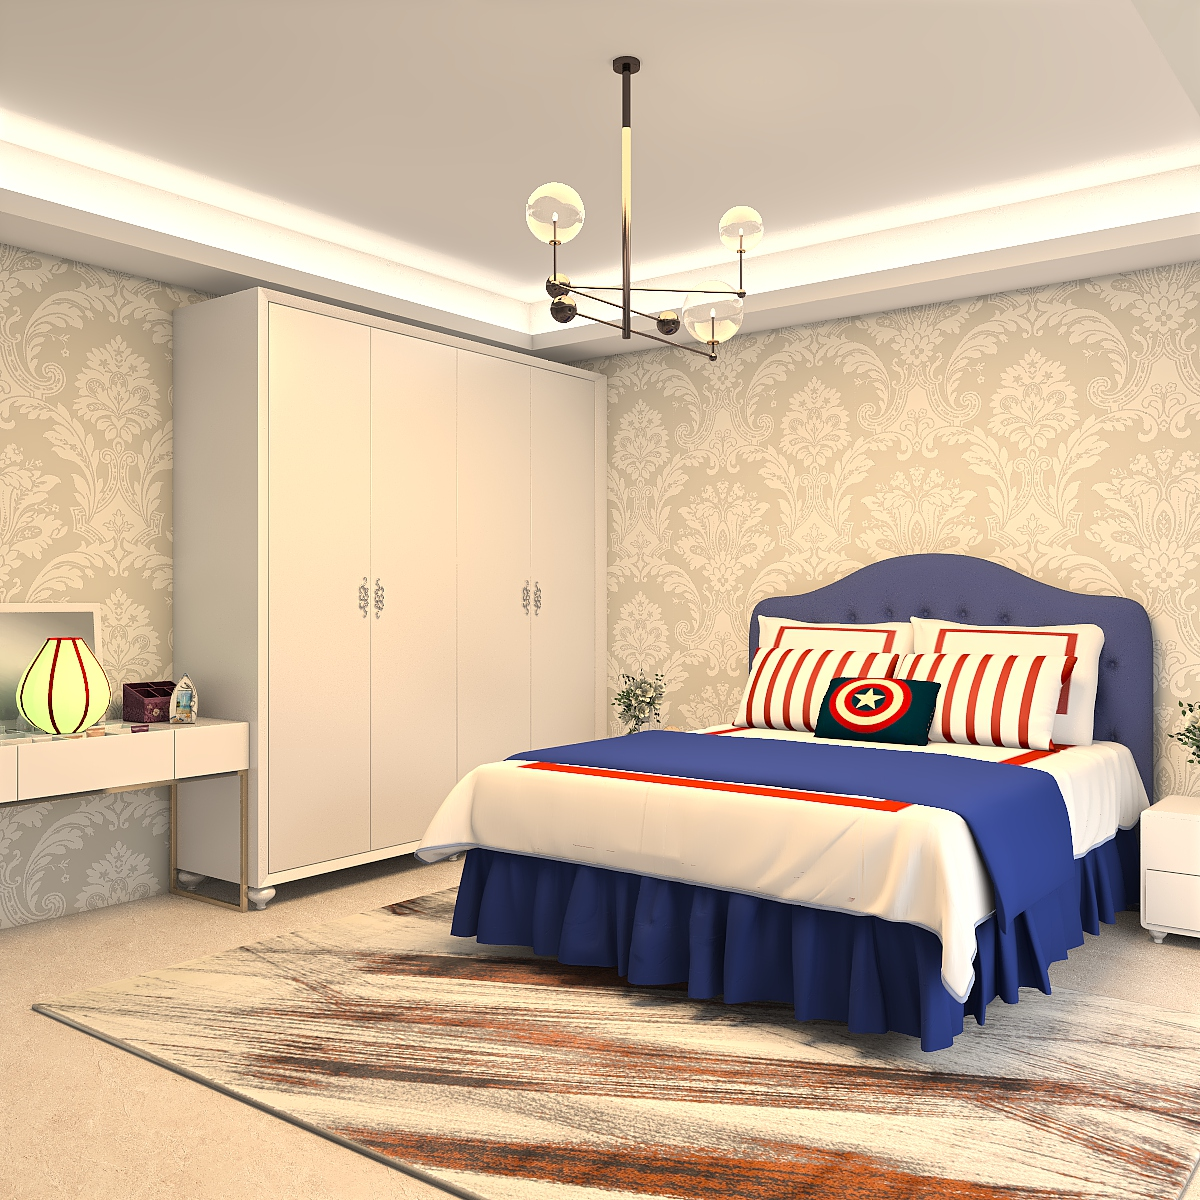
\includegraphics[width=.2\linewidth,valign=m]{/Users/apple/OVGU/Thesis/code/3dReconstruction/report/images/realistic_images_relatedwork/3dfront_1} &
    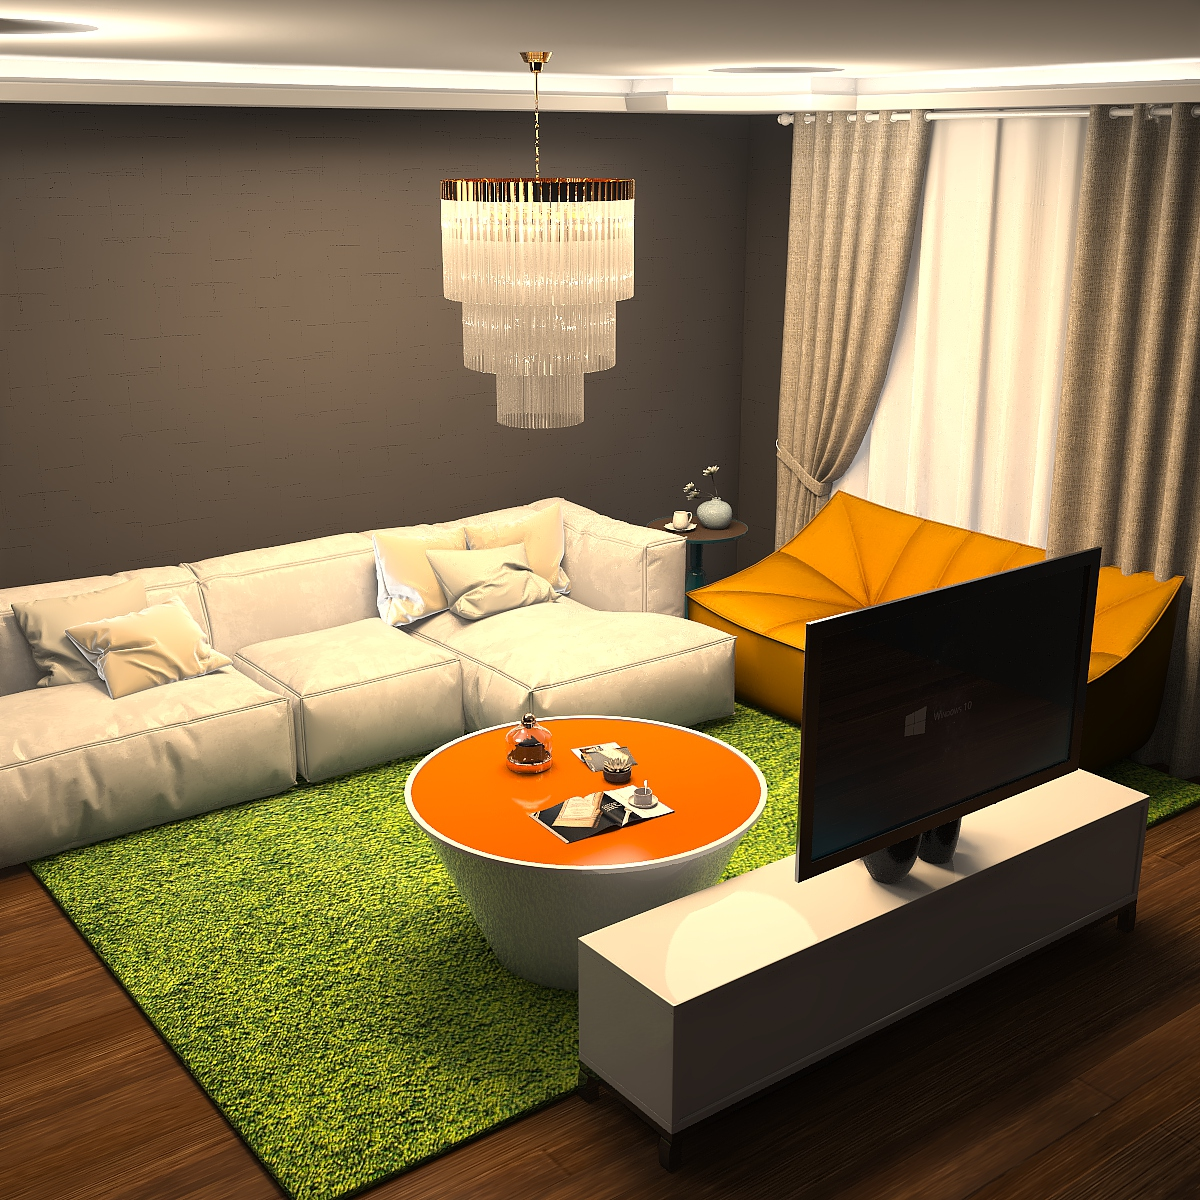
\includegraphics[width=.2\linewidth,valign=m]{/Users/apple/OVGU/Thesis/code/3dReconstruction/report/images/realistic_images_relatedwork/3dfront_2} &
    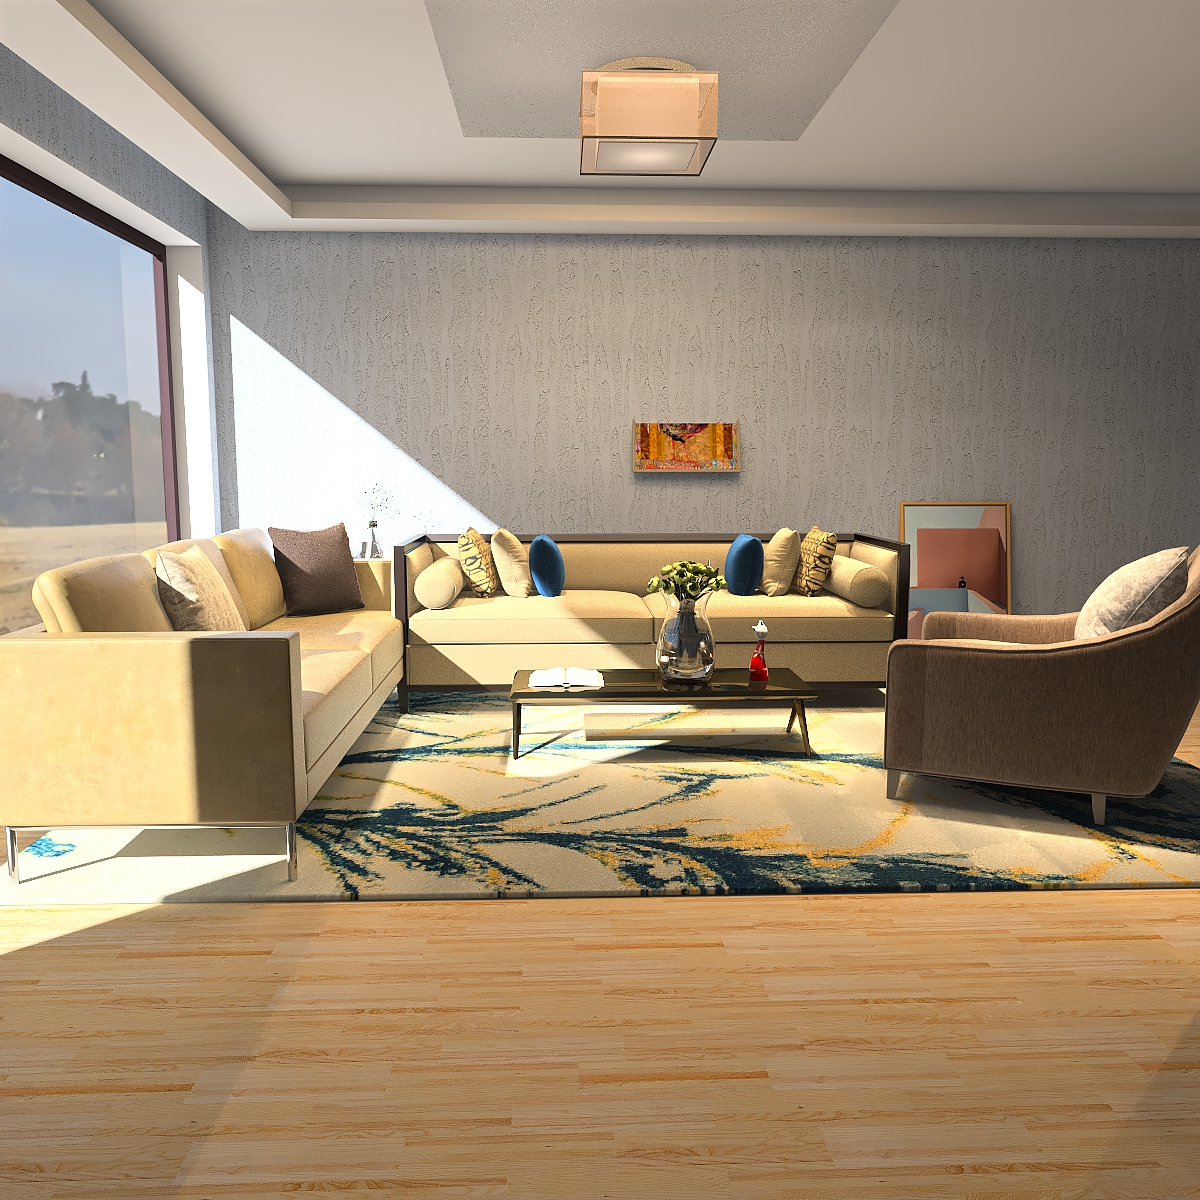
\includegraphics[width=.2\linewidth,valign=m]{/Users/apple/OVGU/Thesis/code/3dReconstruction/report/images/realistic_images_relatedwork/3dfront_3}\\

    AI2THOR & 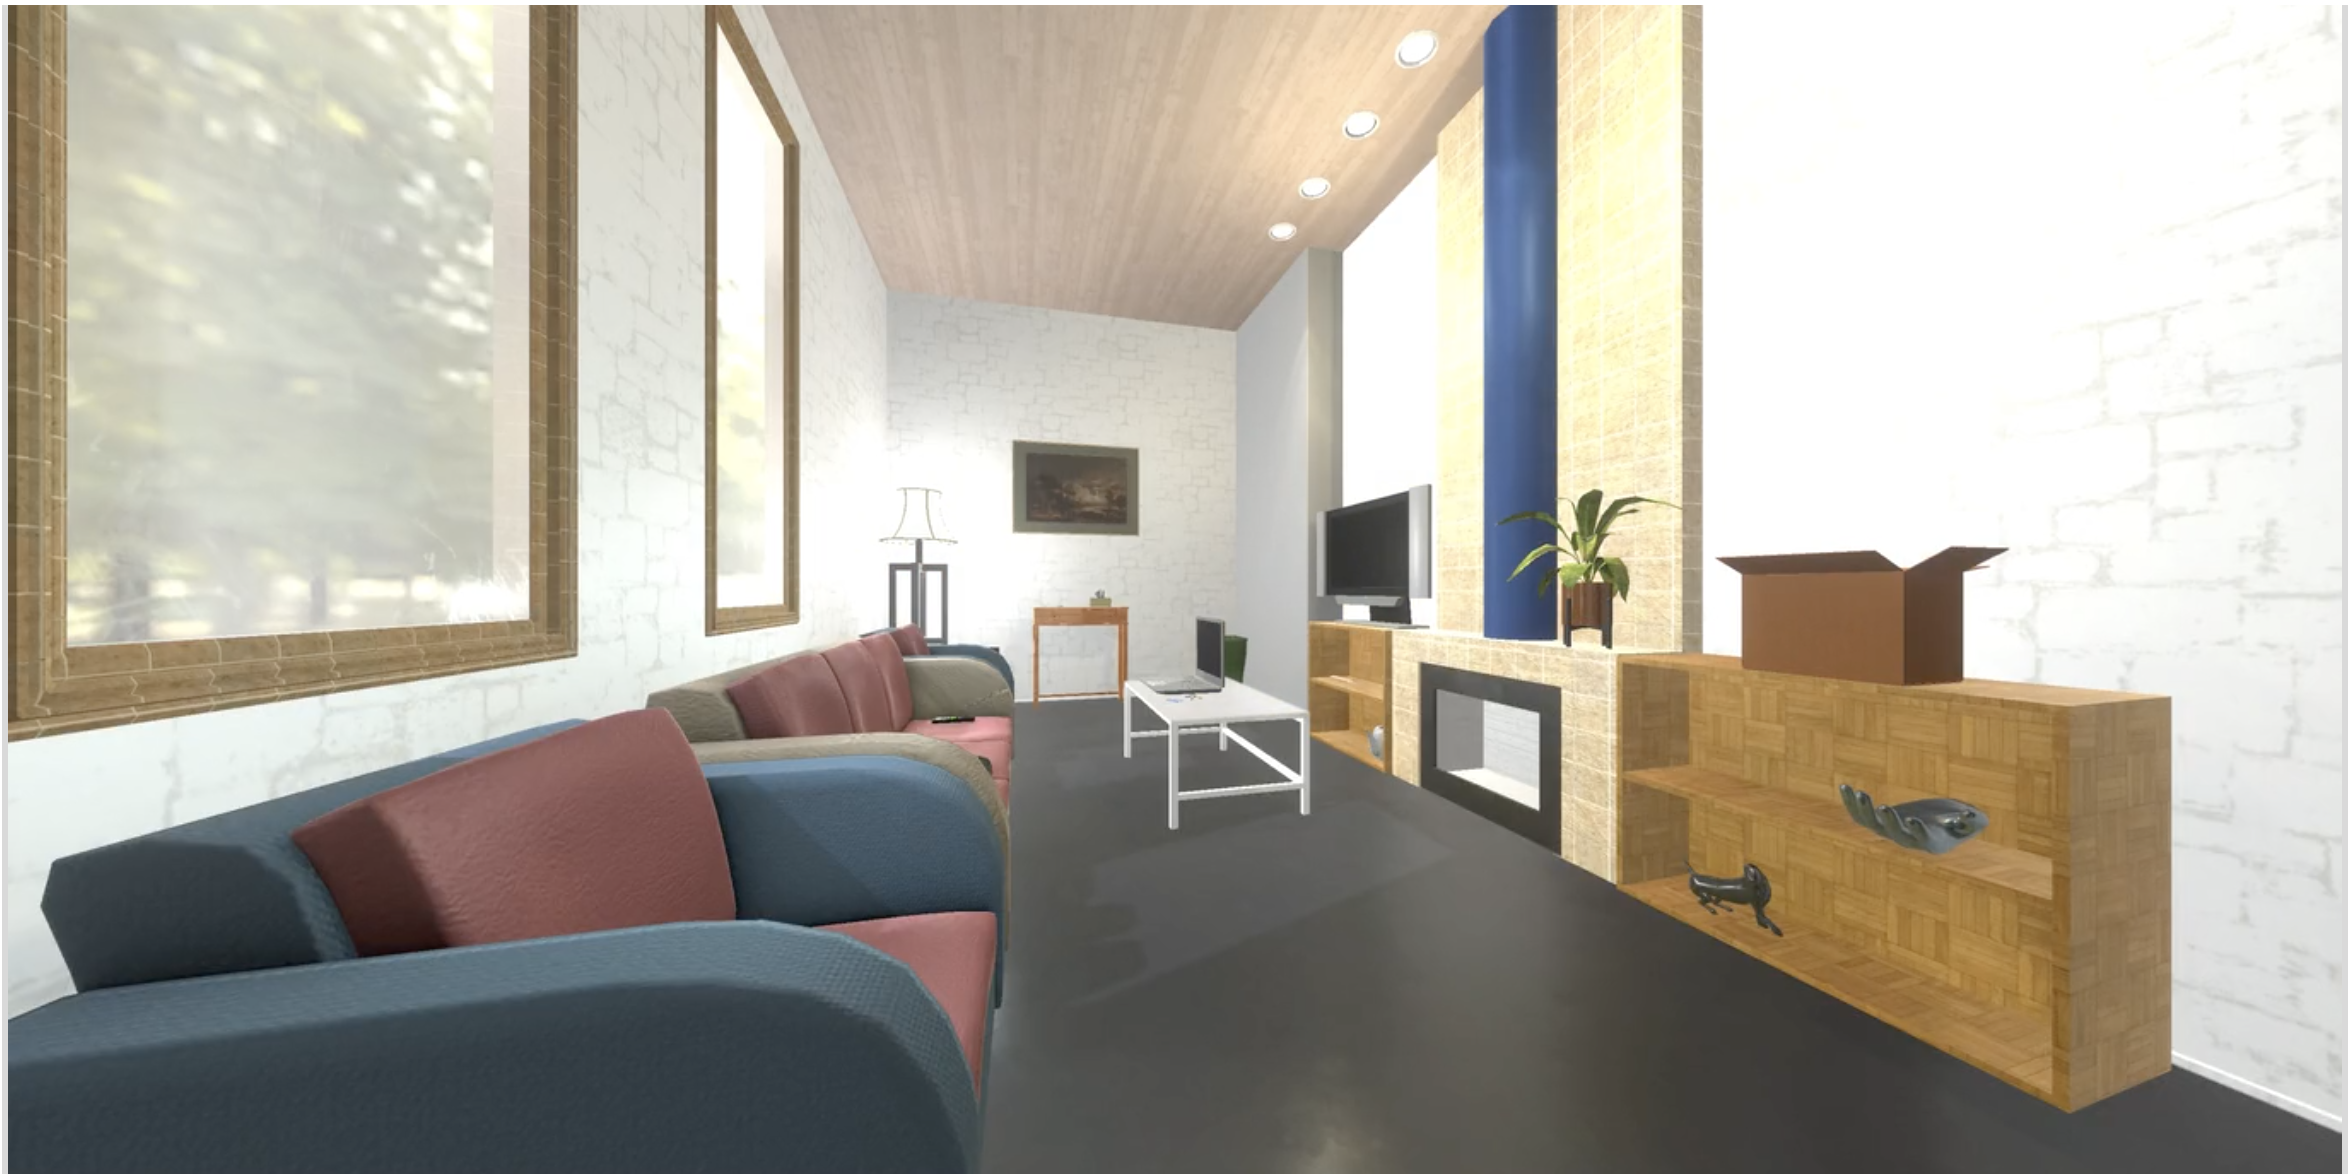
\includegraphics[width=.2\linewidth,valign=m]{/Users/apple/OVGU/Thesis/code/3dReconstruction/report/images/realistic_images_relatedwork/ai2thor_01} &
    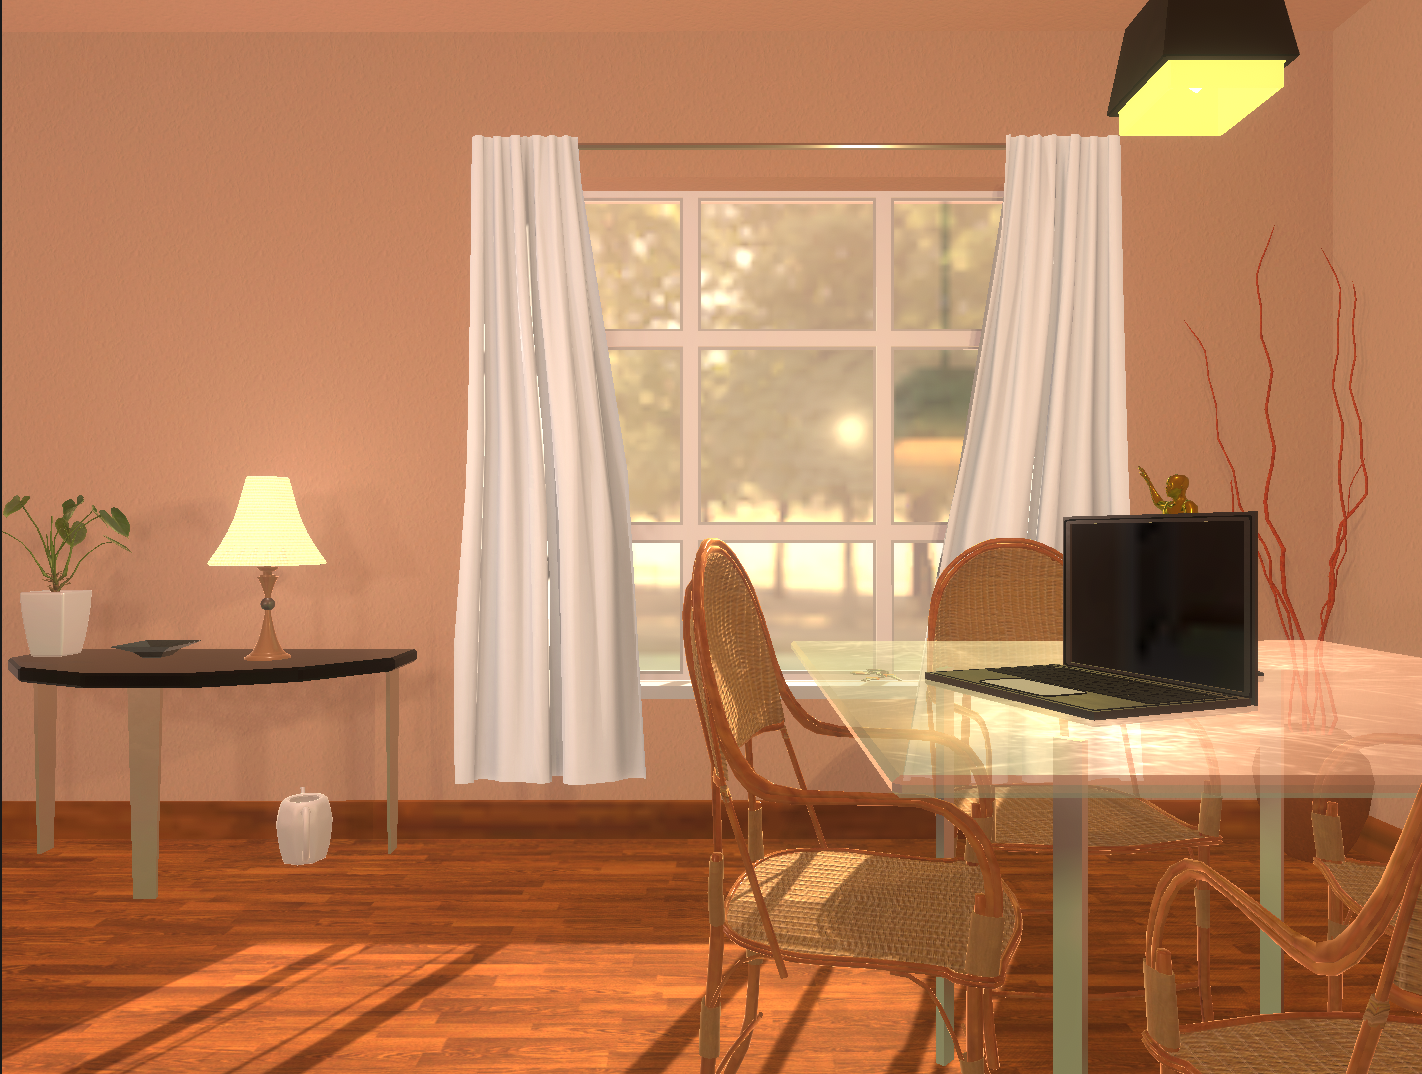
\includegraphics[width=.2\linewidth,valign=m]{/Users/apple/OVGU/Thesis/code/3dReconstruction/report/images/realistic_images_relatedwork/ai2thor_02} &
    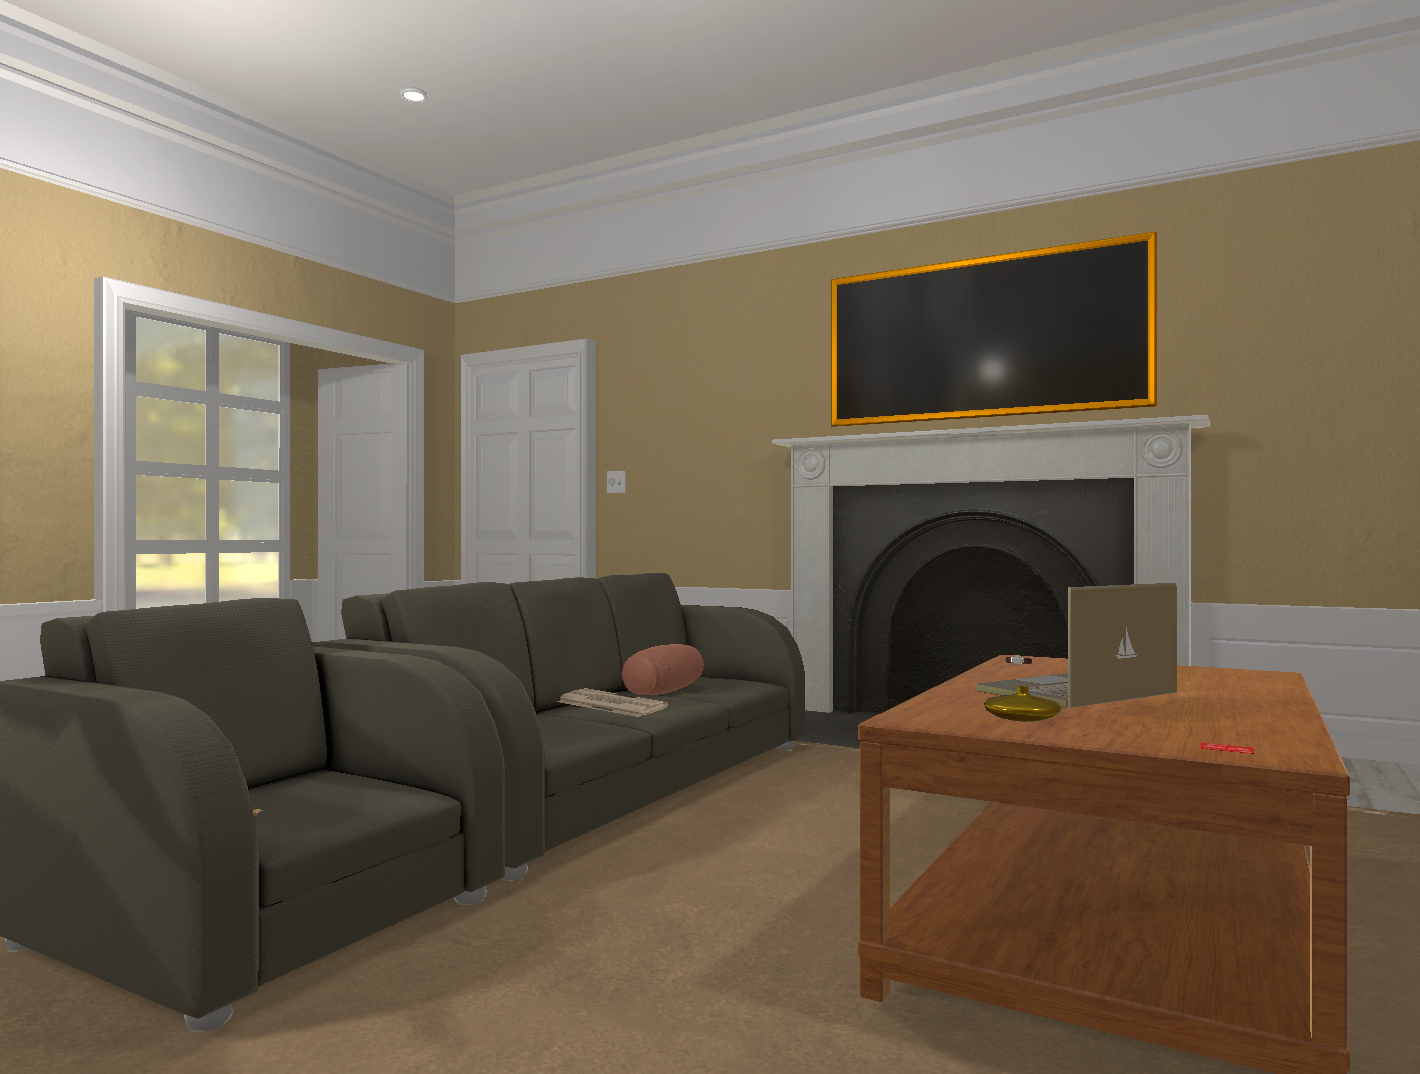
\includegraphics[width=.2\linewidth,valign=m]{/Users/apple/OVGU/Thesis/code/3dReconstruction/report/images/realistic_images_relatedwork/ai2thor_03}\\

    Hypersim & 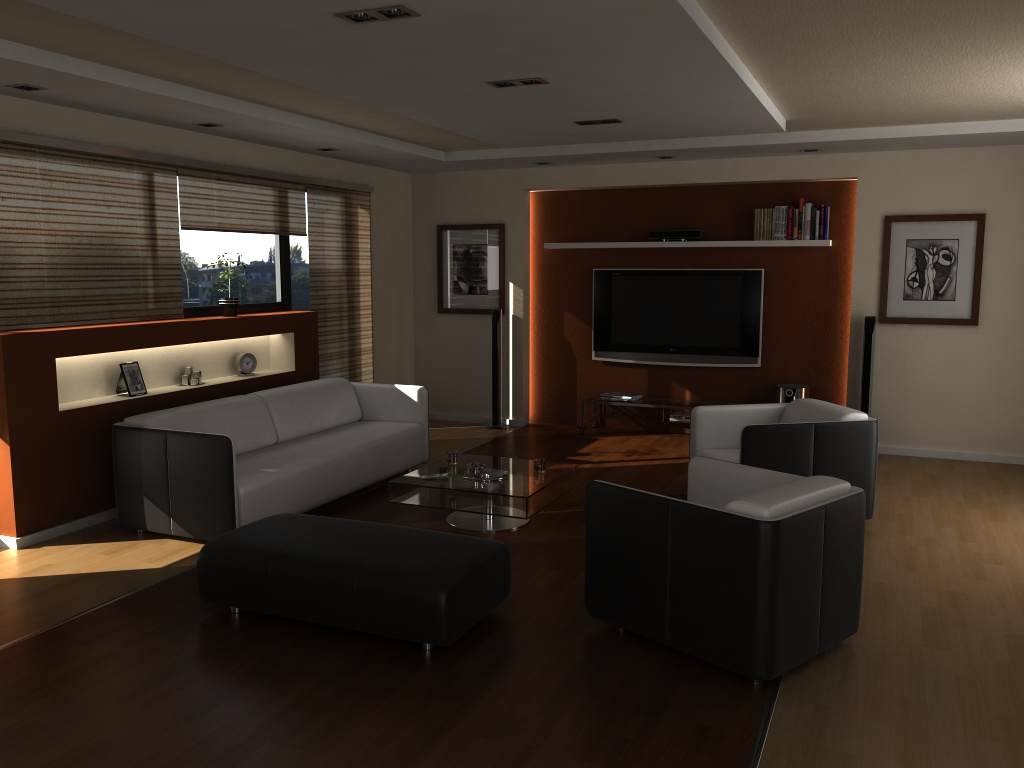
\includegraphics[width=.2\linewidth,valign=m]{/Users/apple/OVGU/Thesis/code/3dReconstruction/report/images/realistic_images_relatedwork/hypersim_01} &
    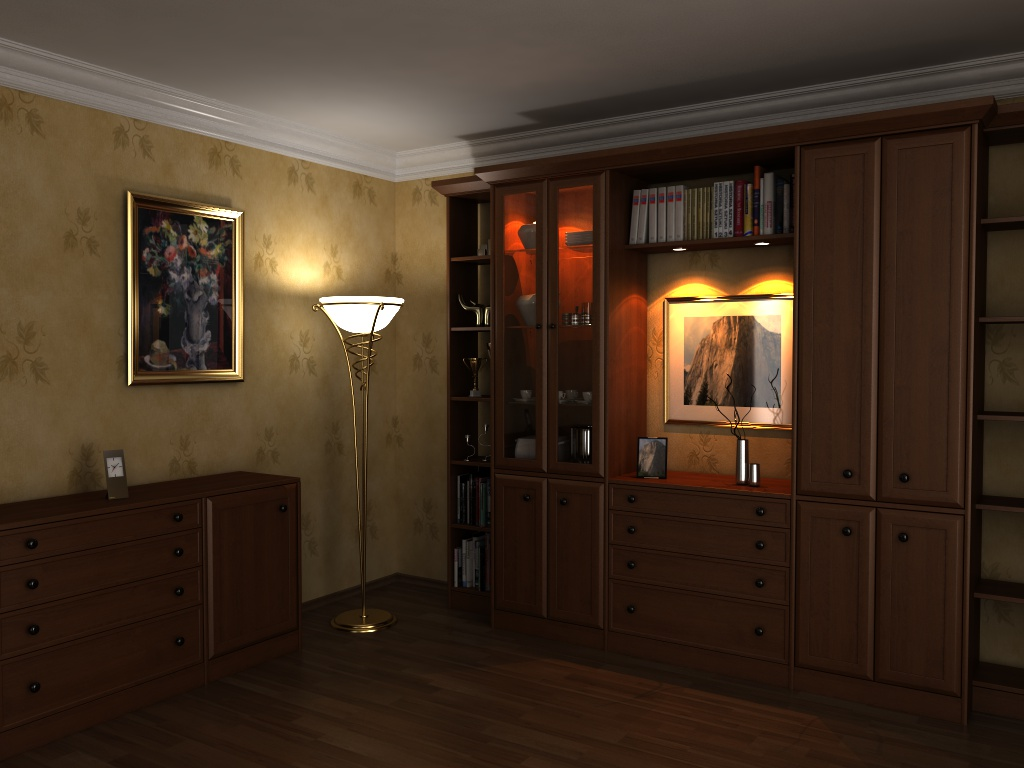
\includegraphics[width=.2\linewidth,valign=m]{/Users/apple/OVGU/Thesis/code/3dReconstruction/report/images/realistic_images_relatedwork/hypersim_02} &
    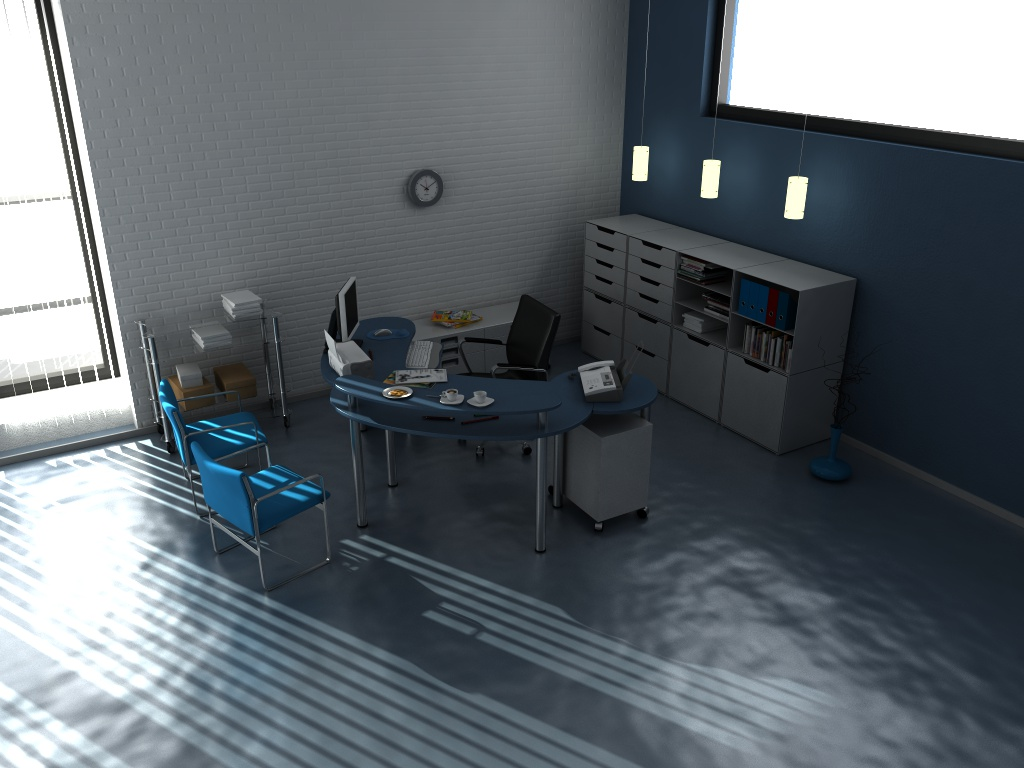
\includegraphics[width=.2\linewidth,valign=m]{/Users/apple/OVGU/Thesis/code/3dReconstruction/report/images/realistic_images_relatedwork/hypersim_03}\\

    InteriorNet & 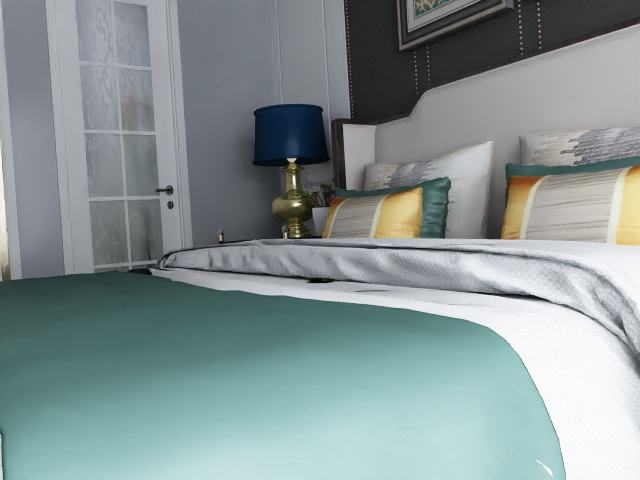
\includegraphics[width=.2\linewidth,valign=m]{/Users/apple/OVGU/Thesis/code/3dReconstruction/report/images/realistic_images_relatedwork/interiornet_01} &
    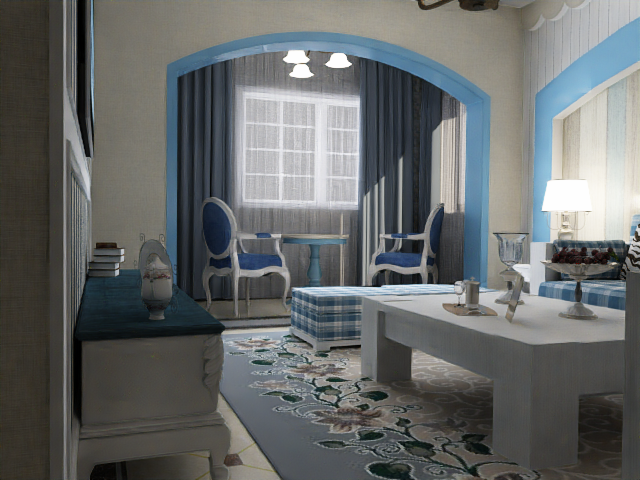
\includegraphics[width=.2\linewidth,valign=m]{/Users/apple/OVGU/Thesis/code/3dReconstruction/report/images/realistic_images_relatedwork/interiornet_02} &
    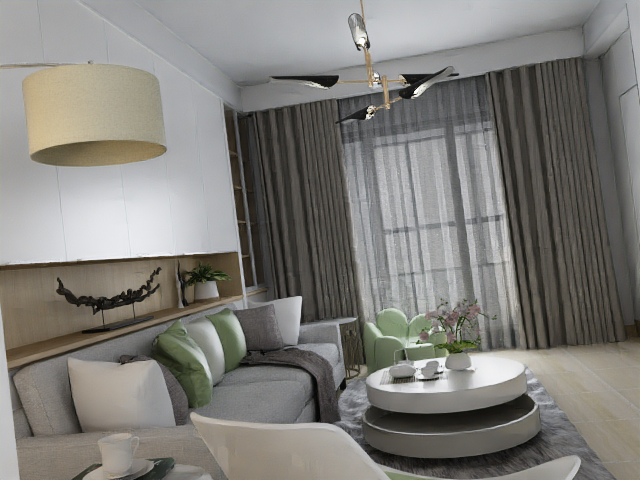
\includegraphics[width=.2\linewidth,valign=m]{/Users/apple/OVGU/Thesis/code/3dReconstruction/report/images/realistic_images_relatedwork/interiornet_03}\\

    OpenRooms & 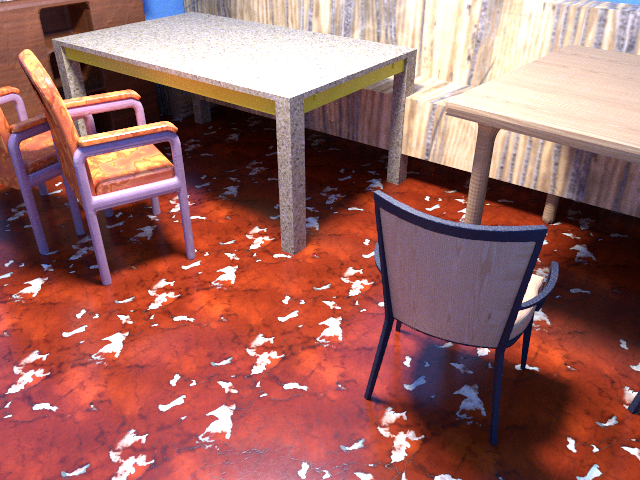
\includegraphics[width=.2\linewidth,valign=m]{/Users/apple/OVGU/Thesis/code/3dReconstruction/report/images/realistic_images_relatedwork/openrooms_01} &
    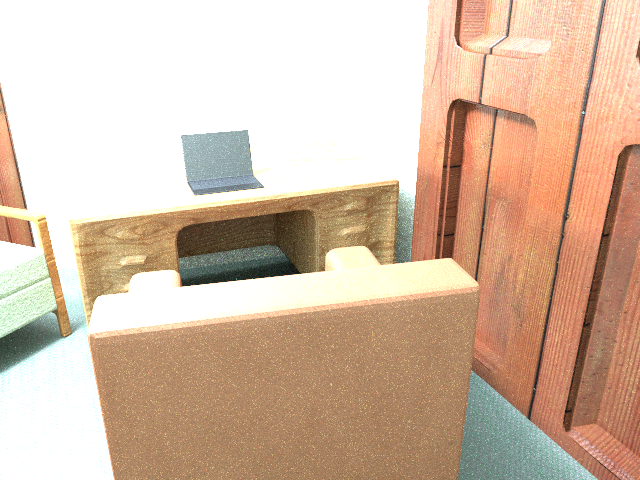
\includegraphics[width=.2\linewidth,valign=m]{/Users/apple/OVGU/Thesis/code/3dReconstruction/report/images/realistic_images_relatedwork/openrooms_02} &
    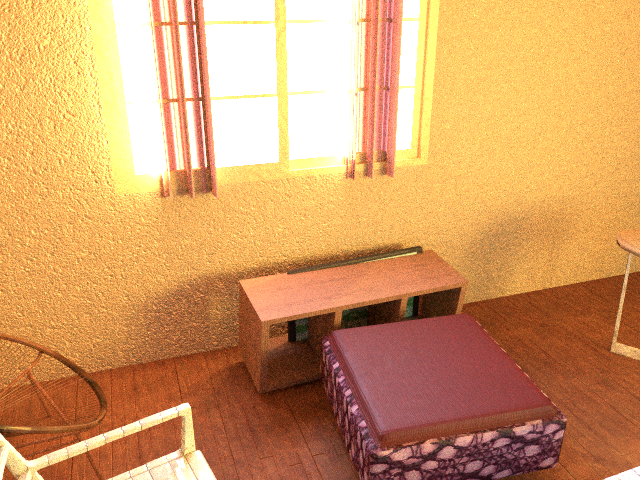
\includegraphics[width=.2\linewidth,valign=m]{/Users/apple/OVGU/Thesis/code/3dReconstruction/report/images/realistic_images_relatedwork/openrooms_03}\\

    SceneNet & 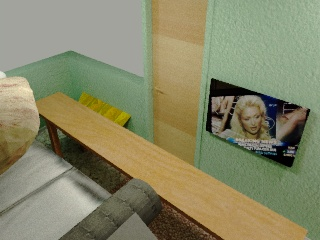
\includegraphics[width=.2\linewidth,valign=m]{/Users/apple/OVGU/Thesis/code/3dReconstruction/report/images/realistic_images_relatedwork/scenenet_1} &
    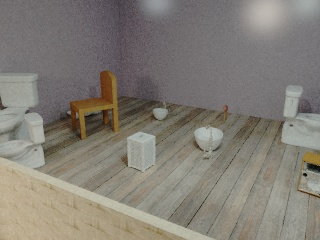
\includegraphics[width=.2\linewidth,valign=m]{/Users/apple/OVGU/Thesis/code/3dReconstruction/report/images/realistic_images_relatedwork/scenenet_2} &
    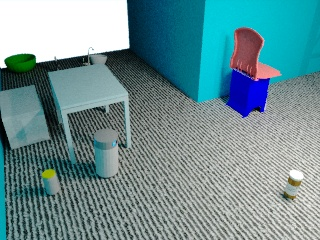
\includegraphics[width=.2\linewidth,valign=m]{/Users/apple/OVGU/Thesis/code/3dReconstruction/report/images/realistic_images_relatedwork/scenenet_3}\\

\end{tabular}
\caption{A collection of photorealistic synthetic datasets. The first column of each row indicates the dataset name followed by randomly selected images from the same dataset.}
\label{fig:photorealistic images comparison}
\end{figure}

\subsection{Tools to create synthetic datasets}\label{subsec:tools-to-create-synthetic}

BlenderProc: Reducing the Reality Gap with Photorealistic Rendering ~\cite{denninger2019blenderproc} is a python based pipeline to create synthetic dataset.
As the name suggests, the key underlying framework is Blender ~\cite{blender}, which is a 3D modelling and rendering package.
Like most of the synthetic data generation tools it provides with rgb, depth maps, normals, semantic segmentation.
Figure ~\ref{fig:Blenderproc samples} is a collection of sample images generated using BlenderPoc.
As far as we searched for synthetic data generation tools, Blenderproc supports maximum number of existing dataset.
Ikea~\cite{Lim2013ParsingIO}, Pix3d~\cite{pix3d}, Shapenet~\cite{chang2015shapenet},3DFront~\cite{Fu20203DFRONT3F} Replica~\cite{Straub2019TheRD}, SunCG~\cite{Xiao2013SUN3DAD} are some of the popular dataset it supports.
It also has some combinations of these datasets like ShapeNet with SunCG or SceneNet.
Even though it supports rendering of Pix3D dataset, the model is rendered without any background.
One extreme advantage of this toolkit, is that it is opensource and hence a wider open community to contribute.

\begin{figure}
    \begin{tabular}{llll}
        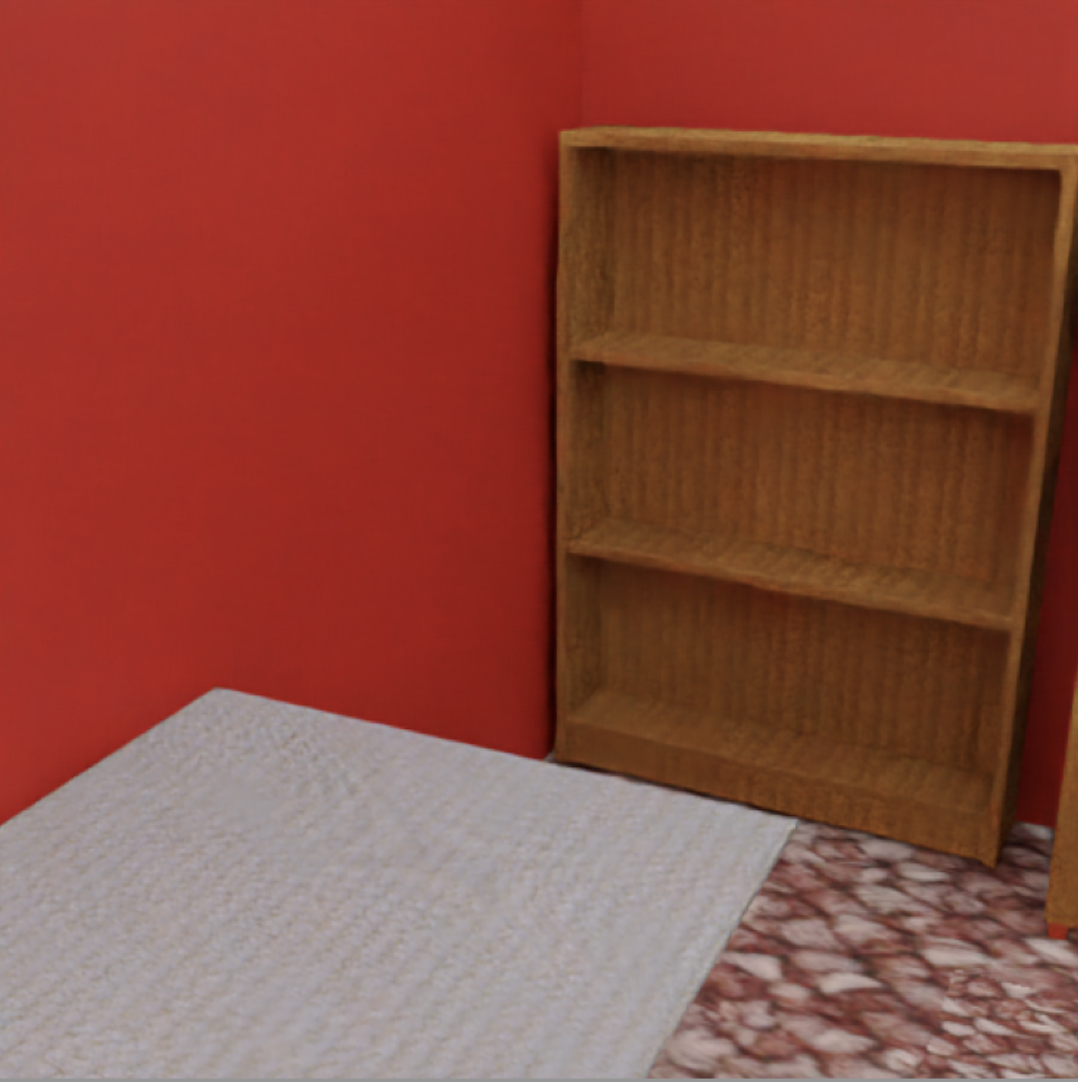
\includegraphics[width=.2\linewidth,valign=m]{/Users/apple/OVGU/Thesis/code/3dReconstruction/report/images/realistic_images_relatedwork/blenderproc_1} &
        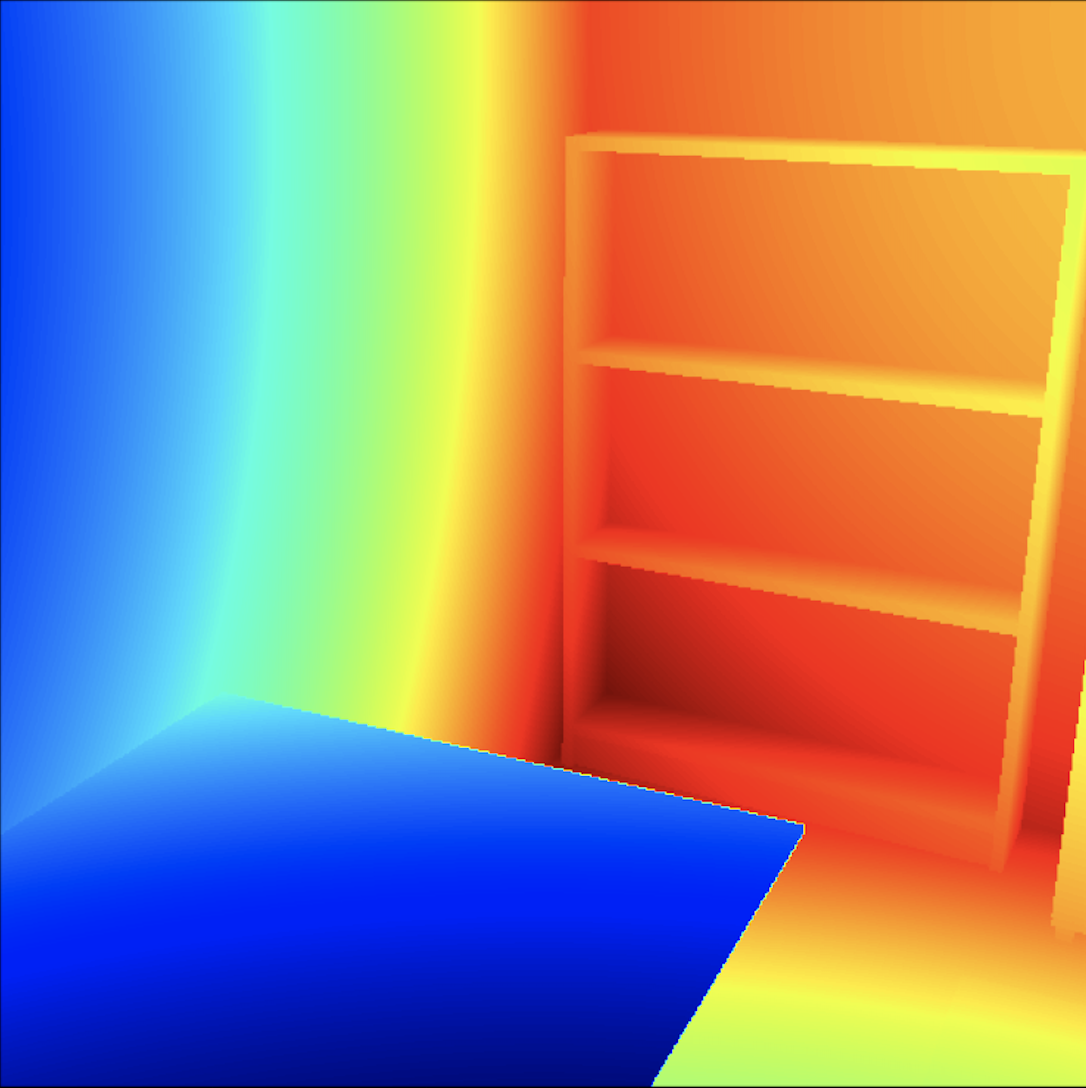
\includegraphics[width=.2\linewidth,valign=m]{/Users/apple/OVGU/Thesis/code/3dReconstruction/report/images/realistic_images_relatedwork/blenderproc_depth_1} &
        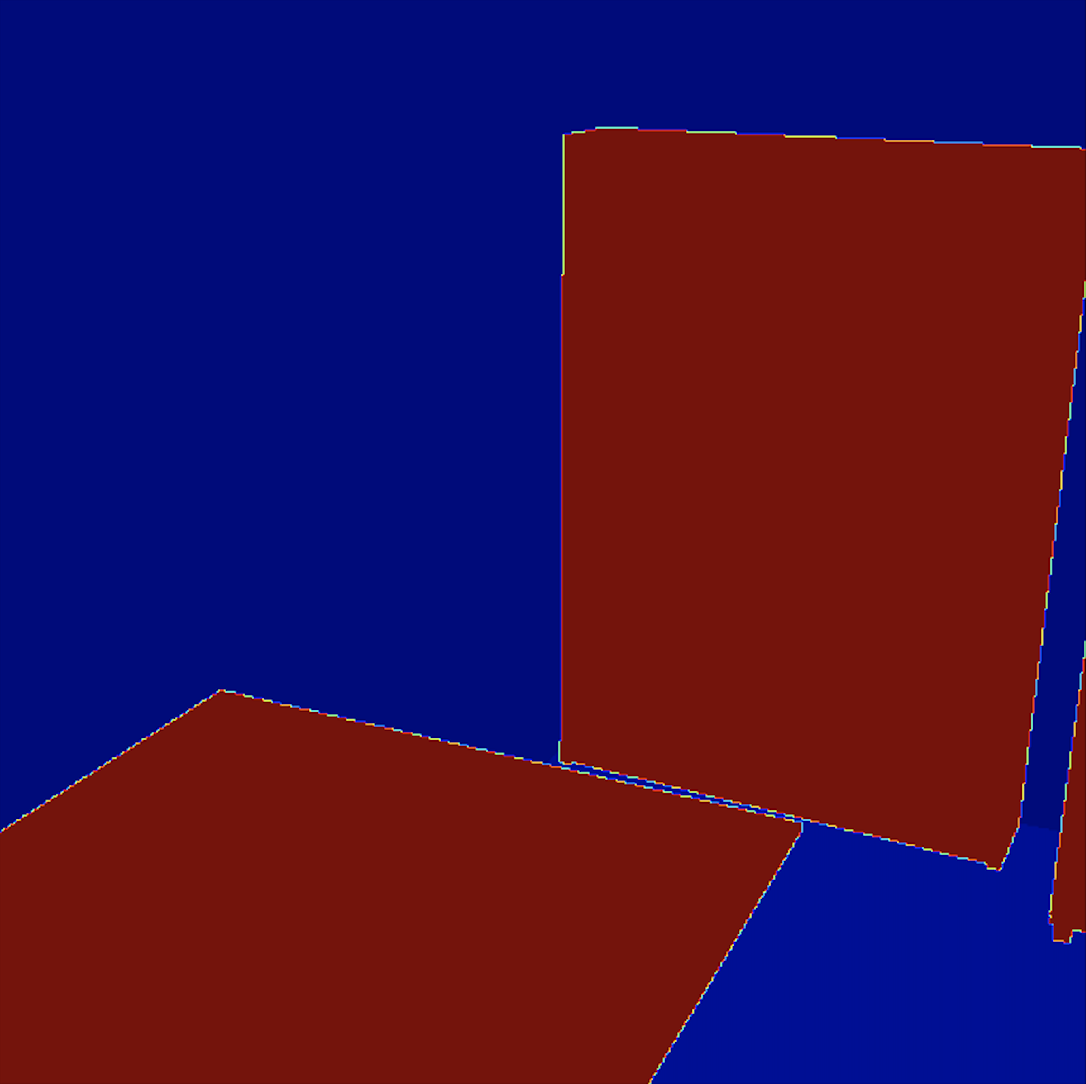
\includegraphics[width=.2\linewidth,valign=m]{/Users/apple/OVGU/Thesis/code/3dReconstruction/report/images/realistic_images_relatedwork/blenderproc_instance_1} &
        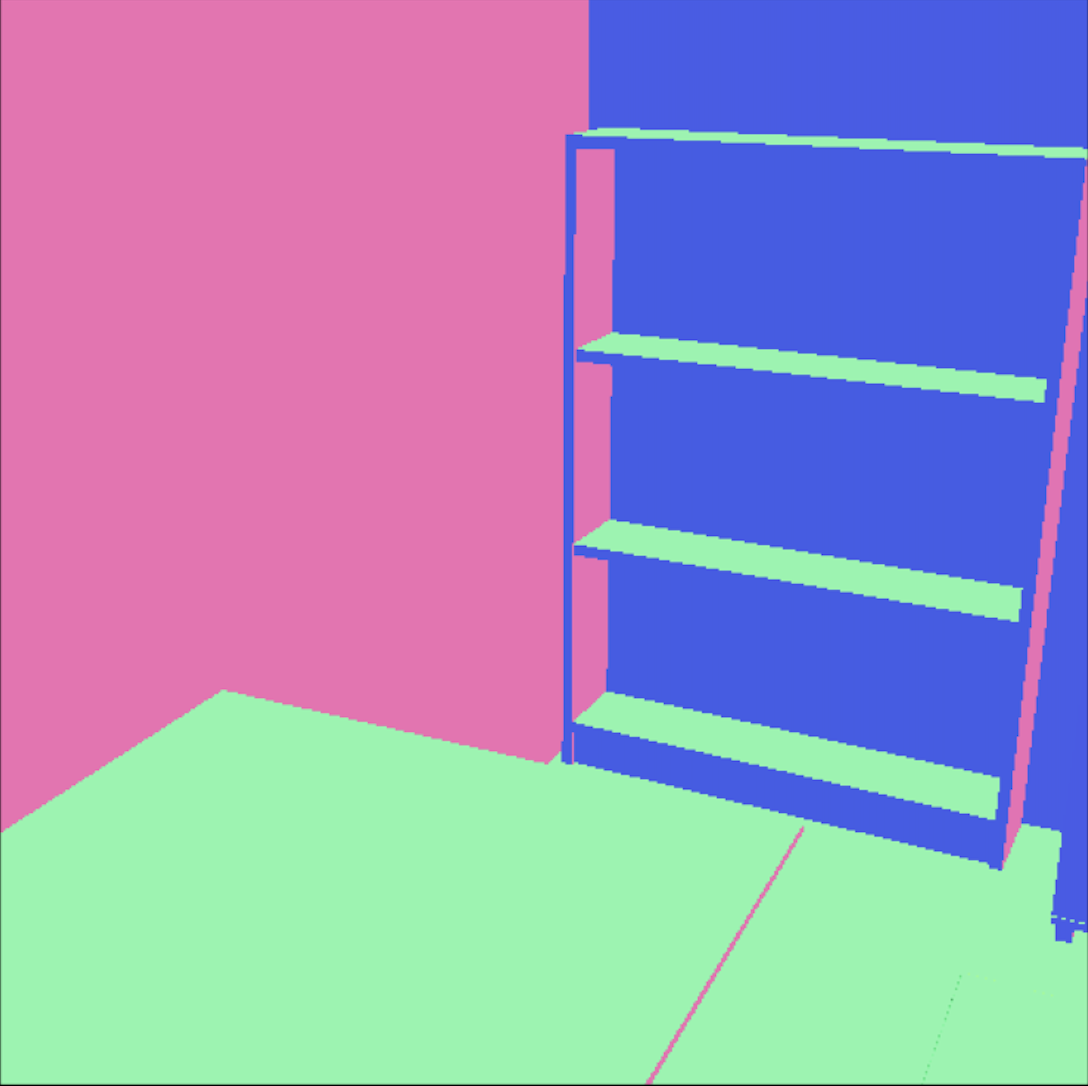
\includegraphics[width=.2\linewidth,valign=m]{/Users/apple/OVGU/Thesis/code/3dReconstruction/report/images/realistic_images_relatedwork/blenderproc_normal_1}\\


        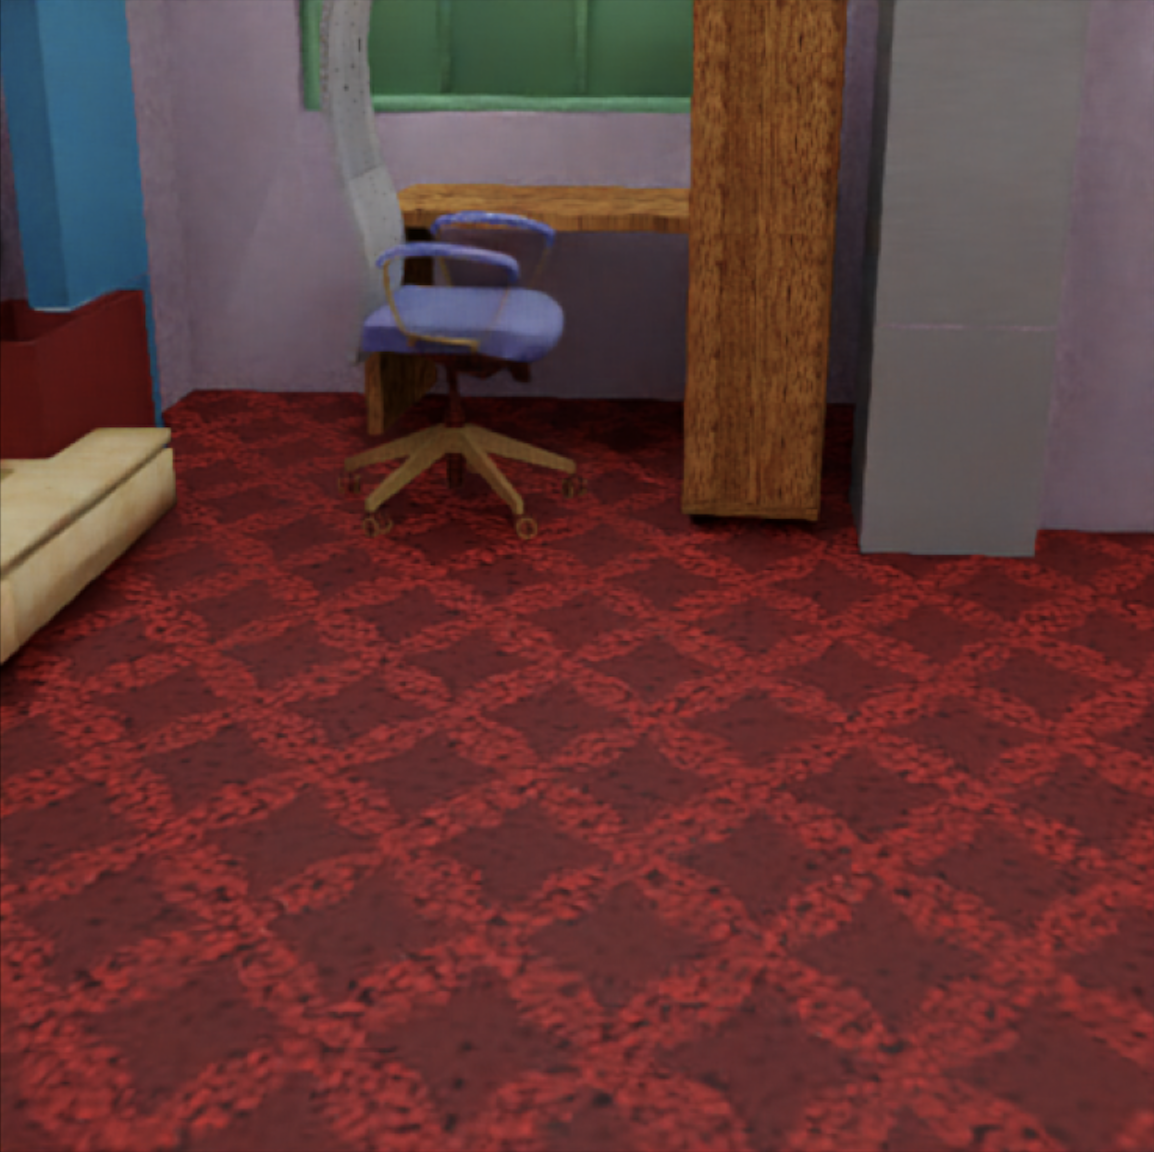
\includegraphics[width=.2\linewidth,valign=m]{/Users/apple/OVGU/Thesis/code/3dReconstruction/report/images/realistic_images_relatedwork/blenderproc_2} &
        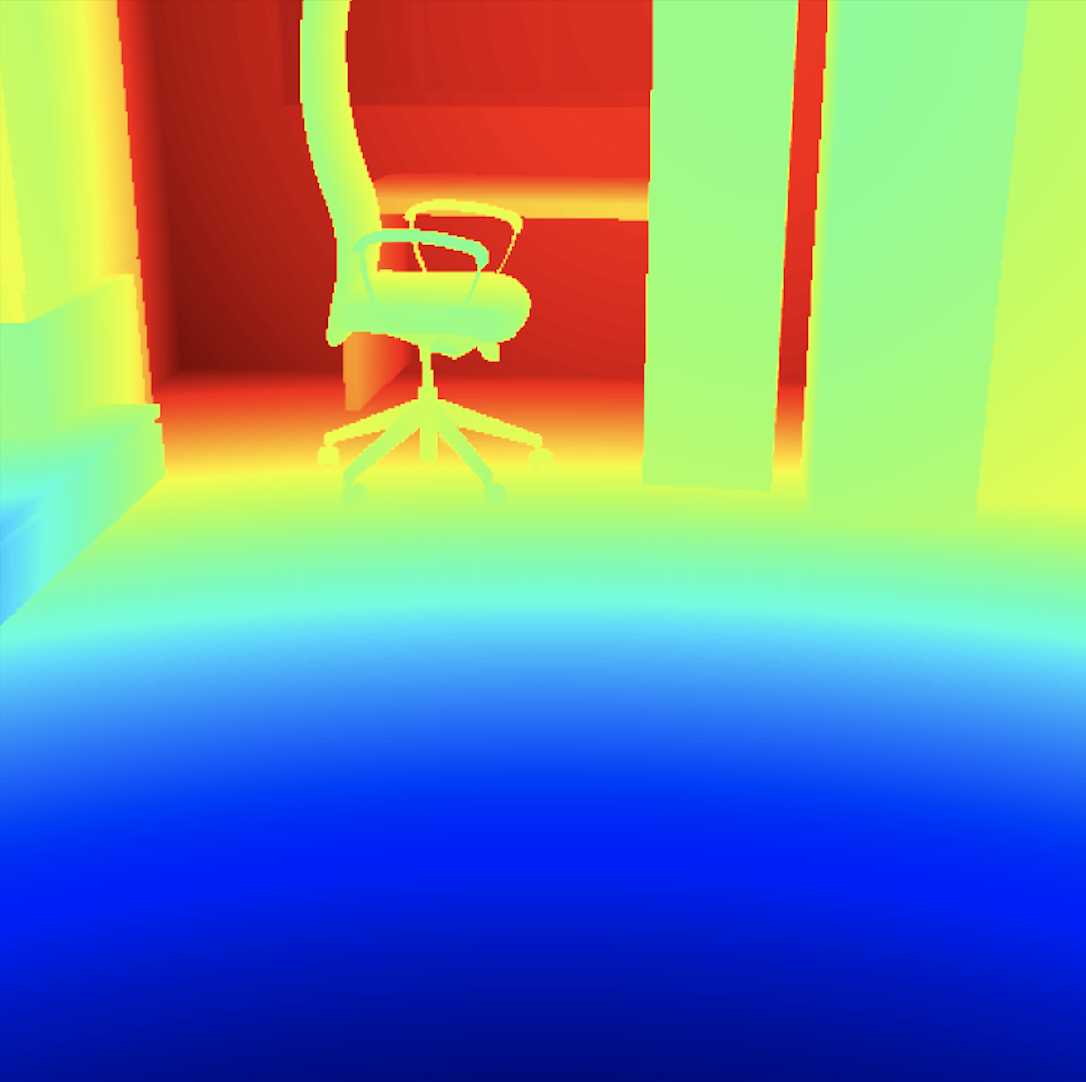
\includegraphics[width=.2\linewidth,valign=m]{/Users/apple/OVGU/Thesis/code/3dReconstruction/report/images/realistic_images_relatedwork/blenderproc_depth_2} &
        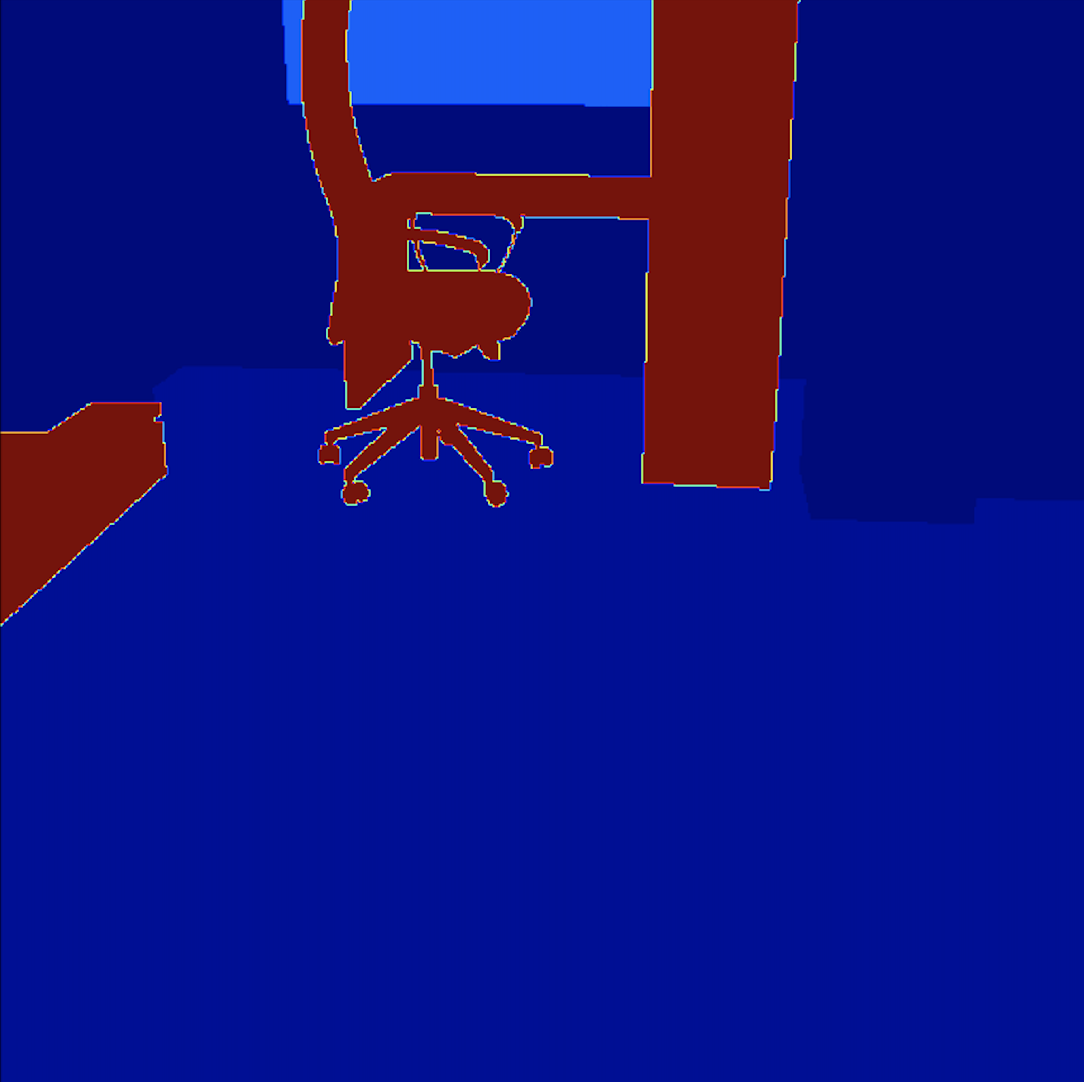
\includegraphics[width=.2\linewidth,valign=m]{/Users/apple/OVGU/Thesis/code/3dReconstruction/report/images/realistic_images_relatedwork/blenderproc_instance_2} &
        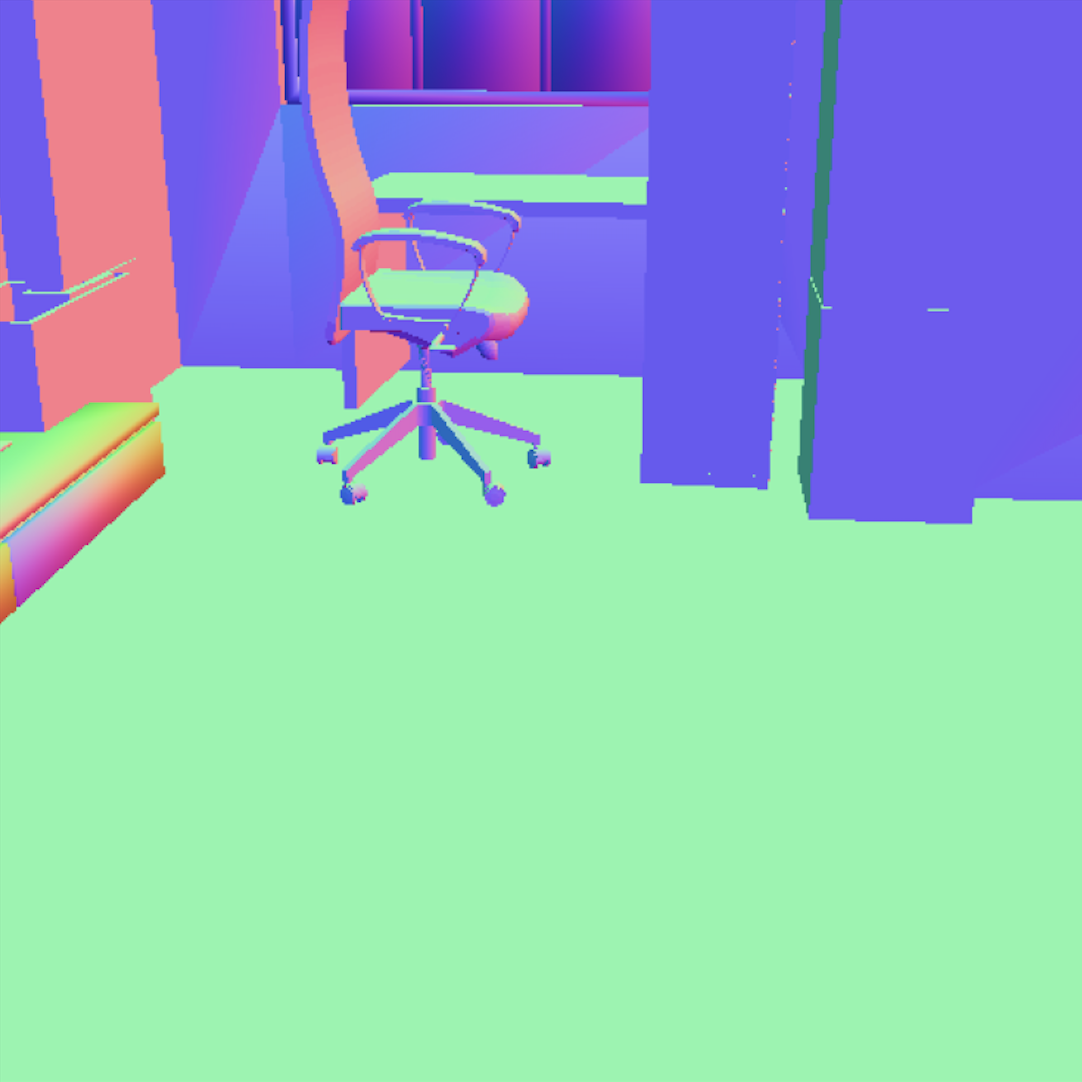
\includegraphics[width=.2\linewidth,valign=m]{/Users/apple/OVGU/Thesis/code/3dReconstruction/report/images/realistic_images_relatedwork/blenderproc_normal_2}\\

%        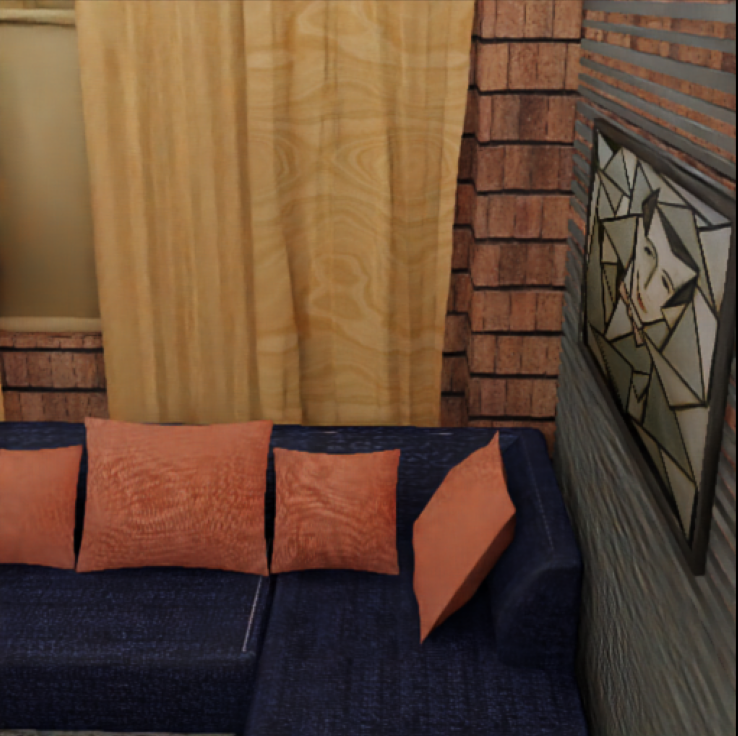
\includegraphics[width=.2\linewidth,valign=m]{/Users/apple/OVGU/Thesis/code/3dReconstruction/report/images/realistic_images_relatedwork/blenderproc_3} &
%        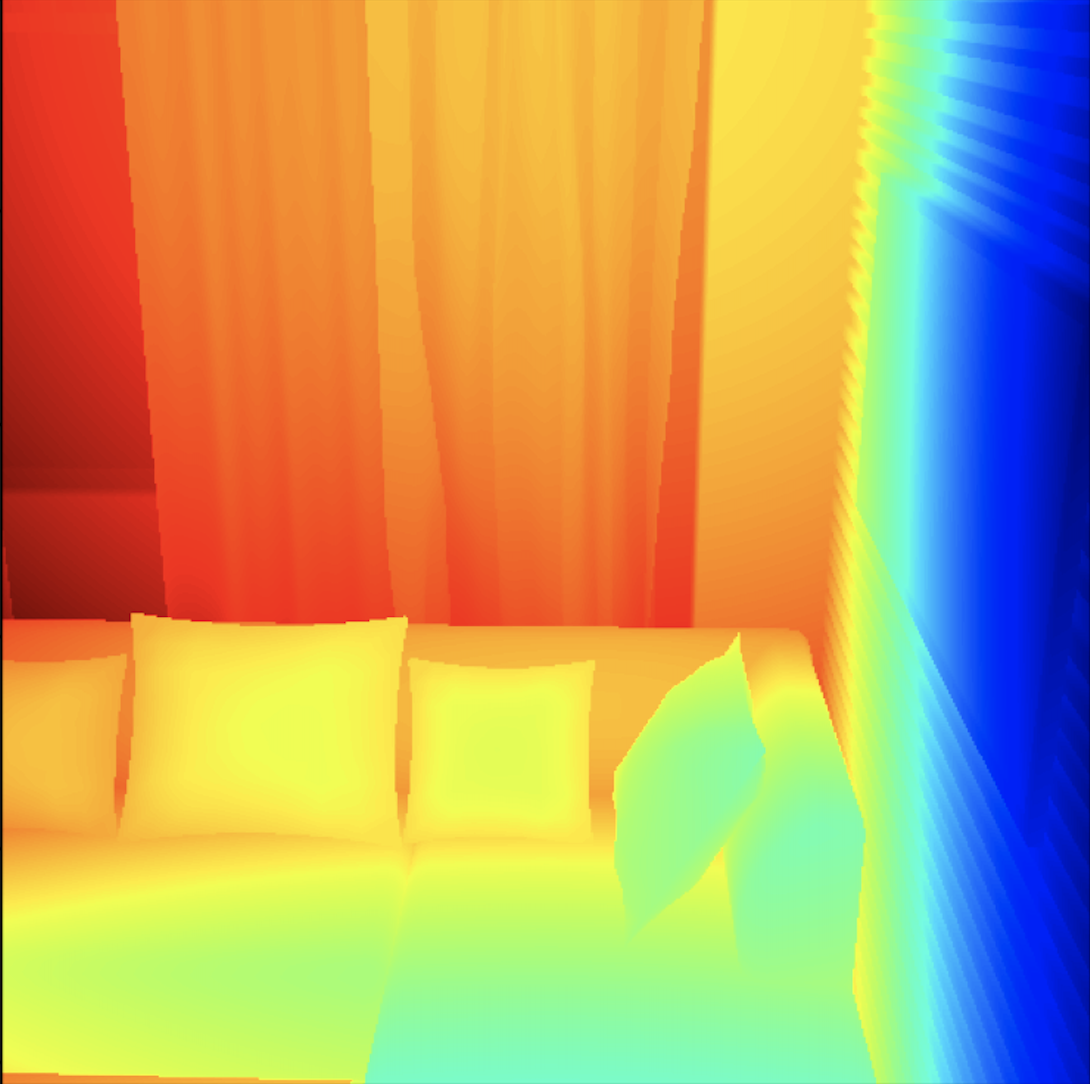
\includegraphics[width=.2\linewidth,valign=m]{/Users/apple/OVGU/Thesis/code/3dReconstruction/report/images/realistic_images_relatedwork/blenderproc_depth_3} &
%        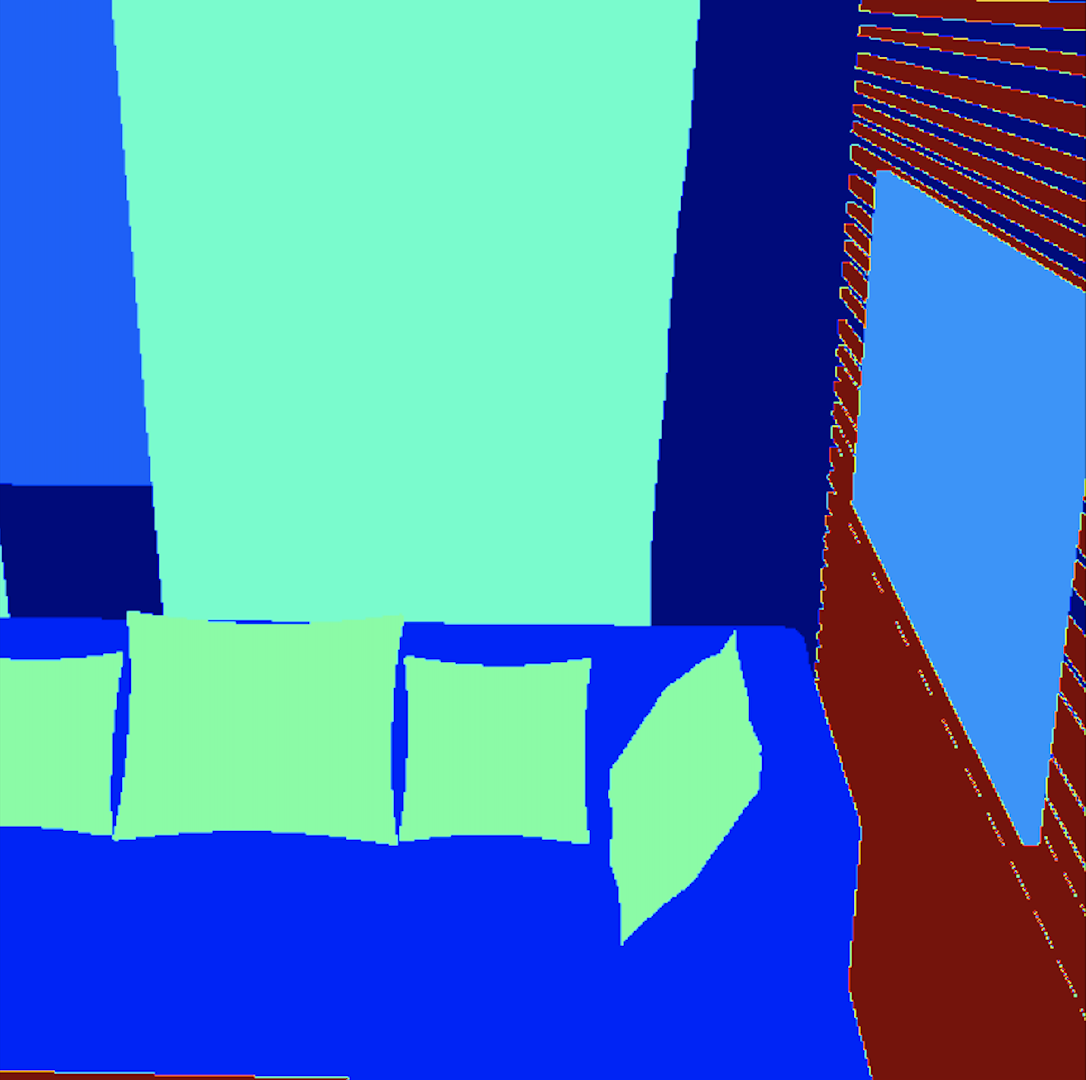
\includegraphics[width=.2\linewidth,valign=m]{/Users/apple/OVGU/Thesis/code/3dReconstruction/report/images/realistic_images_relatedwork/blenderproc_instance_3} &
%        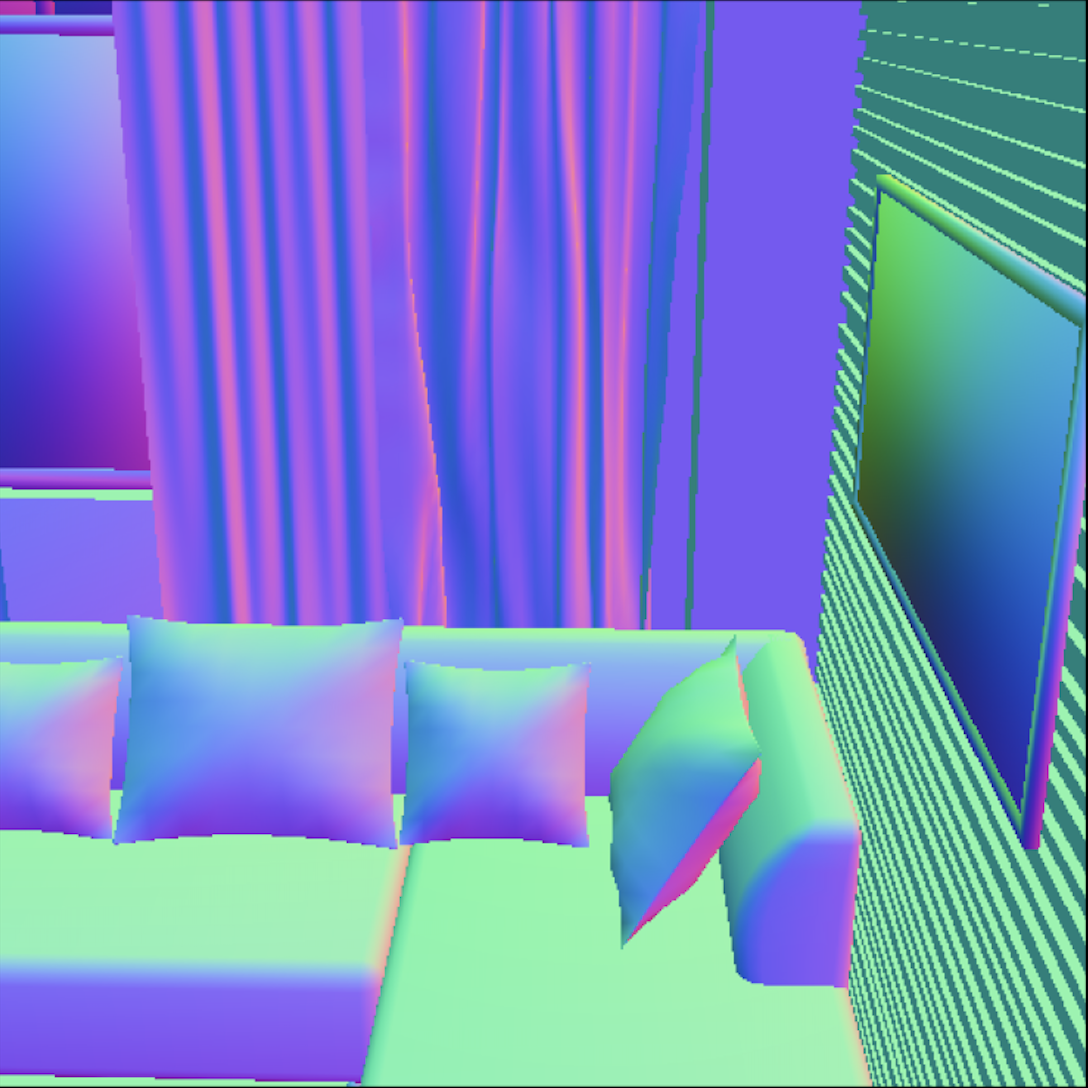
\includegraphics[width=.2\linewidth,valign=m]{/Users/apple/OVGU/Thesis/code/3dReconstruction/report/images/realistic_images_relatedwork/blenderproc_normal_3}\\

    \end{tabular}
    \caption{Sample images created from BlenderProc using SceneNet dataset.(Left to right) RGB images, Depth Maps, Instance Segmenatations and Normals. Each row is an independent sample.}
    \label{fig:Blenderproc samples}
\end{figure}

NVIDIA developed a Deep learning Dataset Synthesizer (NDDS) ~\cite{to2018ndds} in the form of a plugin for Unreal Engine 4(UE4).
The plugin can synthesize images,per-pixel segmentation, depth, object 3D pose, 2D/3D bounding box, keypoints, and custom stencils.
It even supports domain randomisation of objects, lighting, camera position, poses and textures.
Leveraging the asynchronous-multithreaded frames, data was generated at high rates(50-100 Hz) for Falling Things (FAT) ~\cite{tremblay2018falling} dataset.

"SynthDet: An end-to-end object detection pipeline using synthetic data" ~\cite{synthdet2020}, is an open source project supported by Unity technologies using Unity Engine.
This is an ML pipeline which uses 63 categories of common objects(example: cereal box, cady, cartons, etc) as synthetic objects to generate 2D bounding boxes.
This project was highly influenced by ~\cite{hinterstoisser2019annotation}, where in they use synthetic 3D models with randomised background to generate synthetic dataset for object detection task.
With domain randomisation the author of ~\cite{hinterstoisser2019annotation} proved that no real data or mixed training is required for Deep Learning model to perform significantly.

UnrealCV ~\cite{qiu2017unrealcv} is open source project built upon Unreal Engine 4 (UE4) ~\cite{unrealengine}).
It supports some pre-built indoor architectures available on the asset store, which are unfortunately paid versions.
Along with this limitation, the plugin only creates depthmaps, normals and segmentation masks, with no mapping to 3D models.
Another tool based on Unreal engine is UnrealROX+\cite{martinezgonzalez2021unrealrox}.
This pluggin design is based on UnrealCV and provides similar data.

\section{State of the art for 3d-reconstruction}\label{sec:state_of_the_art}

3D reconstruction task is on the rise with improvement in technologies like Augmented and virtual reality.
Scene understanding becomes important for these technologies to succeed.
As discussed in ~\ref{sec:Volumetric representation}, 3D models can be represented as voxels,meshes or point clouds.
Each of the representations have been explored for reconstruction and this section explores some approaches.

The task can either be applied to \b{multi-view, or a single view image}.
~\cite{Kar2017LearningAM, choy20163d, Yang_2019, huang2018deepmvs, Paschalidou2018RayNetLV, Xie_2019, Xie_2020}, are architectures based on multiple input images of same images from different views to learn the underlying 3D structure.
~\cite{Kar2017LearningAM, choy20163d} are architectures based on Recurrent Neural Networks (RNN) and have the disadvantage of memory, long-term dependencies and long inference time.
~\cite{Yang_2019, huang2018deepmvs, Paschalidou2018RayNetLV} explore different ways of pooling(attentional, max and average pooling respectively) to aggregate the feature vectors from different views.
The pooling method tend to capture only partial information with loss in detailing.

For single-view reconstruction we have architectures like ~\cite{wu2017marrnet,z-gan, Yang_219, wu2018learning, popov2020corenet}.
~\cite{wu2017marrnet} predicts the 3D structure by estimating 2.5D properties like surface normals, segmentation and depths.
~\cite{wu2018learning} is extension of MarrNet which proposes a network to preserve the naturalness of the surface.
Inspired by generative models~\cite{Goodfellow2014GenerativeAN,kingma2014autoencoding}, many 3D reconstruction architectures were published ~\cite{z-gan, Yang_219,wu2017learning,Lunz2020InverseGG}.
Both ~\cite{Xie_2019, Xie_2020} also have the capability to predict 3D structure from a single view image.

To overcome the memory issues caused by 3D voxels many new architectures have also been proposed
~\cite{tatarchenko2017octree,Richter2018MatryoshkaNP,Mescheder2019OccupancyNL,Gkioxari2019MeshR, wang2018pixel2mesh,groueix2018atlasnet,pan2019deep}.
These are approaches that are based out of oct-tree, meshes, occupancy of voxel, etc.
Occupancy networks are a implicit way of representing 3D surface as decision boundary using network as a deep learning classifier.
For mesh-based reconstruction, a template mesh such as an ellipsoid is deformed to get the structure of 3D model.
For the Oct-tree based reconstruction, as the name itself suggest, instead of 3D voxels the models are discretized in Oct-Tree representation.
This further makes it memory and compute efficient providing higher resolution than 3D voxel representation.

Supervision is another factor to consider for 3D reconstruction tasks.
There are method based on \b{3D-Supervision or 2D-Supervision}.
~\cite{Xie_2019,Xie_2020,wu2017marrnet,groueix2018atlasnet,pan2019deep, chen2019learning} are few of the 3D-supervision based architecture.
For all these architectures it is necessary to either have the 3D voxel grid or 3D mesh for supervised training.
For models described in ~\cite{Lunz2020InverseGG,henderson2019learning}, the 3D reconstruction only needs 2D supervision like silhouette,
One might argue that for 3D supervision we need large number of 3D models designed and created by professional artists.
With the advent of Virtual and Augmented realities, 3D models are which are available to public are increasing exponentially, which might resolve the issue.


\section{Mitigating domain shift}\label{sec:mitigating_domain_shift}


In ~\cite{nowruzi2019real}, the author tries to find how much of real data is required with synthetic dataset to increase the performance of object detection task.
A study was conducted by training various object detection models on mixed data containing different ratios of real and synthetic dataset.
The four ratios considered for mixed training were, 0\%, 90\%, 95\%, 97.5\% of synthtic data to real data.
Another study was conducted by fine tuning a model pre-trained on a synthetic dataset with different quantity of real dataset.
They observed that fine-tuning with limited real dataset is better than mixed training with synthetic dataset.

The idea of domain randomisation is that among the set of training images from synthetic dataset, real images appears to be one of the variations.
Thus, testing with real world images should give comparable performance.
~\cite{tobin2017domain} used this principle for small objects detection task used for robotics.
This paper tries different parameters in domain randomisation like lights, camera viewpoints, textures and further combines domain randomisation with domain adaptation.

~\cite{Tremblay2018TrainingDN} explores domain randomisation on real-world object detection.
The author also proposes a new approach of domain randomisation where in random 3d objects called "flying distractors" are randomly placed in the scene,
so that the model learns to ignore objects which are not of interest.
A focused ablation study with individual domain randomisation parameter was also conducted to understand its contribution.
The parameters included lights, textures, data augmentation and flying distractor as mentioned above.

~\cite{prakash2020structured} introduces Structured domain randomisation, where in the structure and context is preserved for the problem at hand while creating synthetic images.
Example: A road is randomly placed with parameters like curvature, lighting and camera position.
With this as context, the pedestrian walk, road lanes, etc are generated.
After these 2 steps, the objects such as cars, cyclists, houses, buildings are placed in the scene.
As ablation study, the author changes domain randomisation parameters and checks the performance on car detection task.

~\cite{georgakis2017synthesizing} proposes a domain randomisation based synthetic images generation for detection of objects found in kitchen.
The objects are cropped and placed on the background with semantic information and geomety with proper scale.
Similar to the above works, here to the author provides ablation study with different ratios of synthetic to real dataset for mixed training.

Domain randomisation and adaptation techniques are not the only ways to mitigate the domain shift.
With advent of Generative Adversarial Networks~\cite{Goodfellow2014GenerativeAN}, synthetic to real image conversions has become possible and can lead to better performance on given task.
~\cite{Richter_2021, CycleGAN2017, park2020cut,isola2017image, dundar2018domain,Wang2018HighResolutionIS} are some of the successful attempts to reduce the gap between simulated environment and reality.
Intel in ~\cite{Richter_2021} uses GTA V dataset with G-buffers(depth, normals, segmentations,Albedo, glossiness, etc.) to enhance the photorealism of synthetic images.
~\cite{park2020cut} uses patchwise contrastive loss so that the content of input image is retained.
The loss is minimised such that corresponding patches retain high mutual values.

Another interesting way to reduce domain gap is using domain adversarial training ~\cite{ganin2016domainadversarial}.
Along with the task in observation, a branched network from the feature extractor is used as a classifier for the domains.
This acts like a multi-learning tasks where feature extractor is the common branch, where in one branch learns to perform a specific task like segmentation or classification, where as the other branch classifies if the dataset is real or synthetic.
~\cite{pinheiro2019domainadaptive} implements the same principle on much complex 3D reconstruction task by predicting voxels and classifying the image domain.

